\chapter{多项式的四则运算}

我们已经学习了一次方程和一元二次方程的解法,总结其要点就是:设未知数、列方程式、进而解方程.从运算的角度上看,其基本原理就是:把未知数当作具有数系运算通性的符号,与已知数一样参加运算,进而再运用数系运算通性去求出所设未知数.这种含有未知数的算式的运算,就是解代数方程的基本功.把这些运算系统化,就是本章的主要内容多项式的四则运算.

\section{单项式与多项式}
\subsection{单项式}
由己知数及未知数符号$x,y,\ldots$的方幂相乘,所得到的式子,叫做\textbf{单项式}.例如:
$8x,\; 9x^2,\; -2x^4,\; \frac{1}{2}x^7,\; -\frac{3}{7}x^{32},\; 0.618xy^2,\; -\sqrt{2}x^{121},\; 7x^2y,\; -\sqrt{7}xyz,\; \frac{3}{4}x^2y^3z$, 以及$-\frac{\sqrt{3}}{5}mt,\; \sqrt{\frac{1}{3}}x^2y^3zt$等都是单项式.

在单项式中,未知数符号前面的数字因数叫做这个单项式的\textbf{系数};未知数符号叫做单项式的\textbf{元};所含不同未知数的个数,就叫这个单项式的\textbf{元数};而所含各元乘方指数的总和,就叫做这个单项式的\textbf{次数}.例如,以上所举各单项式的系数,元数,次数分别如表1.1所示.


今后,我们就以单项式的元数,次数为准来称呼每一个单项式.例如:
$-2x^4$称为一元四次单项式,$0.618xy$与$7xy$
都称为二元三次单项式等.

由于2可以看成$2x^0$,$-\sqrt{5}$可以看成$-\sqrt{5}y^0$等,因而,单独一个不等于0的数,也是一个单项式,只不过这样的单项式的次数都为零次.


所以,一般地说,任一个非零数$a$,都是单项式的特例,我们叫做\textbf{零次单项式}.例如:
$2,-\sqrt{5}, 0.3,-3\sqrt{2},-7\frac{1}{2}$等,都是零次
单项式.
\begin{table}
    \caption{}
    \begin{center}
        \begin{tabular}{cccc}
            \hline
            单项式&        系数& 元数&        次数 \\
            \hline
            $8x$& 8& 一元 & 1次\\
            $9x^2$& 9& 一元 & 2次\\
            $-2x^4$& $-2$& 一元 & 4次\\
            $\frac{1}{2}x^7$& $\frac{1}{2}$& 一元 & 7次\\
            $-\frac{3}{7}x^{32}$& $-\frac{3}{7}$& 一元 & 32次\\
            $0.618xy^2$& 0.618 & 二元& 3次  \\
            $-\sqrt{2}x^{121}$& $-\sqrt{2}$ & 一元& 121次     \\
             $7x^2y$ & 7 & 二元& 3次    \\
              $-\sqrt{7}xyz$ & $-\sqrt{7}$ & 三元& 3次     \\
              $\frac{3}{4}x^2y^3z$  & $\frac{3}{4}$ & 三元& 6次   \\
            $-\frac{\sqrt{3}}{5}mt$  & $-\frac{\sqrt{3}}{5}$ & 二元& 2次   \\
            $\sqrt{\frac{1}{3}}x^2y^3zt$  & $\sqrt{\frac{1}{3}}$ & 四元& 7次    \\
            \hline
        \end{tabular}
    \end{center}
\end{table}



又由于数0可以看成:
\[0\cdot x^0, 0\cdot x, 0\cdot x^2, \ldots , 0\cdot x^n, \ldots\]
所以,对于“零”这个特殊的数,我们就叫做\textbf{零单项式}.零单项式是单项式中唯一的\textbf{次数不定的单项式}.尽管它有多种形式的写法,但\textbf{每种写法中系数都是0}.因而,通常还是用“0”表示零单项式.

综上所述,单项式包括:
\begin{center}
    \begin{tikzpicture}
        \node (A) at (-2,0){单项式};
        \node (B) at (1,1){非零单项式};
        \node (C) at (1,-1){零单项式};
        \node (D) at (4,2){零次单项式};
        \node (E) at (4,0){非零次单项式};
    \draw(A)--(B);
    \draw(A)--(C);
    \draw(D)--(B);
    \draw(E)--(B);
    
    \end{tikzpicture}
\end{center}

\begin{ex}
  \begin{enumerate}
      \item 指出下列各单项式的系数、元数及次数:
      \[x^8,\qquad -x^4y,\qquad 3x^5,\qquad -1.41xyz, \qquad \sqrt{7}x^7 \]
      \[-\frac{1}{\sqrt{2}}xy,\qquad -\sqrt{3},\qquad -x^2y^2z^2,\qquad \frac{22}{7},\qquad 0 \]
      \item 什么是零单项式?它与零次单项式有什么差别?
  \end{enumerate} 
\end{ex}

如果在几个单项式中,不管它们的系数是不是相同,只要它们所含的未知数相同,而且各相同未知数的指数都对应相等,那么,这几个单项式就叫做\textbf{同类单项式}.简称\textbf{同类项}.

例如:
$\frac{1}{2}x^2$与$-5x^2$与$\frac{\sqrt{2}}{2}x^2$是同类项.
$\sqrt{5}xy^2$与$-7xy^2$与$\frac{1}{3}xy^2$也是同类项.$\sqrt{2}xyz^2$与$100xz^2y$与$z^2xy$也是同类项.

但是,$5x^3$, $7y^3$与$7z^3$就不是同类项;$-xy$,
$23xy^2$, $51x^2y$与$\frac{1}{2}x^2y^2$都不是同类项.

\begin{ex}
    把下列各单项式,按同类项分成各个组.你能分出几组来?
\[-7,\qquad  6x,\qquad \frac{1}{2}x^3y,\qquad \sqrt{2},\qquad -xyz,\qquad -0.5yx^3 \]
\[\sqrt{5}zyx,\qquad \frac{x^3y}{5},\qquad 0.1x,\qquad 9yxz,\qquad 10yx^3 \]
\end{ex}



\subsection{多项式}
由有限个单项式的代数和组成的式子,叫做\textbf{多项式}.也就是说,用“$+$”“$-$”号把有限个单项式连结起来所得的式子,就叫多项式.例如:$3x+0.5+2x^2$, $x^3-3x+\sqrt{2}$, $xy-3x+\sqrt{5}y+1$, $-\frac{\sqrt{2}}{7}x^3y^3+2.31x^2-8z$等,
都是多项式.

一个单项式可以看作是多项式的特例,特别是,
\textbf{零单项式}也可以称为\textbf{零多项式}.

多项式就是若干单项式的代数和,而单项式又是一些数与具有数系运算通性的未知数符号的方幂所组
成的.因此,单项式自然也具有数系运算通性,就是说:

\textbf{单项式加、乘满足交换、结合律及分配律};例如:
\begin{equation*}
    5x^2-1+8x=5x^2+8x-1 \tag{交换律}
\end{equation*}
\begin{align*}
(7xy-8y^2)+3xy &=(7xy+3xy)-8y^2 \tag{交换律,结合律}\\
&=10xy-8y^2 \tag{分配律}
\end{align*}

\textbf{单项式0与单项式1具有数0与1的运算特性};例如:
$7x^3+0=7x^3$, $(7x^3)\cdot 0=0$, $7x^3\cdot 1=7x^3$等.

利用单项式运算的通性,特别是运用交换律、结合律和分配律,我们完全可以把一个多项式当中的同类项合并起来,集中成为一项,这就是\textbf{合并同类项}.例如:
\begin{align*}
3x+7x^2-15x &= 7x^2+(3x-15x) \tag{交换律,结合律}\\
&=7x^2+(3-15)x \tag{分配律}\\
&=7x^2-12x
\end{align*}
\[3x^2+\sqrt{3}x^3-\sqrt{2}x^2-2x^3=(3-\sqrt{2})x^2+(\sqrt{3}-2)x^3 \]
\[x^3-2x^2y+y^3+x^2y+1=x^3-x^2y+y^3+1 \]

由此可知,\textbf{合并同类项,就是指同类单项式的相加或相减},其法则是:\textbf{把同类单项式的系数相加或相减,而单项式中的未知数及它们的乘方指数不变}.

对于一元单项式来说,合并同类项,就是一元同类单项式相加或相减,它的法则可以用以下式子表示:
\[\boxed{ax^n +bx^n = (a+b)x^n,\qquad  ax^n -bx^n =(a-b)x^n}\]
其中,$a,b$为单项式的系数,可以是任意的己知实数;$n$为自然数.

\begin{example}
    合并以下各同类项:
    \begin{enumerate}
        \item $x+2x+3x+4x$
        \item $7x^3-2x^3+5x^3+(-0.5)x^3-0.7x^3$
        \item $\sqrt{2}xy^2-xy^2+3xy^2-\frac{\sqrt{2}}{2}xy^2  $
    \end{enumerate}
\end{example}

\begin{solution}
    \begin{enumerate}
        \item $x+2x+3x+4x=(1+2+3+4)x=10x$
        \item $7x^3-2x^3+5x^3+(-0.5)x^3-0.7x^3=(7-2+5-0.5-0.7)x^3=8.8x^3$
        \item $\sqrt{2}xy^2-xy^2+3xy^2-\frac{\sqrt{2}}{2}xy^2=\left(\sqrt{2}-\frac{\sqrt{2}}{2}-1+3\right)xy^2=\left(\frac{\sqrt{2}}{2}+2\right)xy^2$
    \end{enumerate}
\end{solution}

\begin{ex}
    合并以下各同类项:
\begin{enumerate}
    \item (口答):
    \[7x^4+(-9)x^4,\qquad \frac{1}{2}x^3-\frac{1}{8}x^3,\qquad 0.5x^7+\frac{1}{100}x^7,\qquad 81x^{12}-(-3x^4)^3\]
    \[ 9xy^2-xy^2 ,\qquad 4y^2z^2-(-2zy)^2,\qquad 2x^2-\left(-\frac{1}{2}\right)x^2-5x^2,\]\[ 4x^3+(-x)^3-\frac{9}{4}x^3+\left(-\frac{1}{4}\right)x^3 \]
    \item $3xy^3-4y^3x+7xy^3-(-2)xy^3,\qquad ax^n+bx^n+cx^n-dx^n$
\end{enumerate}
\end{ex}

在多项式中,所含不同未知数的个数,称为这个
多项式的\textbf{元数};经过合并同类项以后,多项式所含非零单项式的个数,称为这个多项式的\textbf{项数};多项式合并同类项后,所含各单项式中最高次项的次数,就称为这个多项式的\textbf{次数}.例如:
\begin{itemize}
    \item $3x+0.5+2x^2$就是一元、三项、二次多项式;
    \item $x^3-3x+x^2+\sqrt{2}-x=x^3-3x+\sqrt{2}$(合并同类项),就是一元、三项、三次多项式;
    \item $xy-3x+\sqrt{5}y+1$就是二元四项二次多项式;
    \item $-\frac{\sqrt{2}}{2}x^2y^2 +2.3xz-8z^2$就是三元、三项、五
次多项式.
\end{itemize}

在今后,我们常常把所遇到的多项式,先合并同类项,再以这个多项式的元数、次数为准来称呼这个多项式.例如:
\begin{itemize}
    \item $x^3-3x+\sqrt{2}$ 称为一元三次多项式;
    \item $x^2+x^3-y-x^2=x^3-y$ 称为二元三次多项式.
\end{itemize}
特别是,象$10,\sqrt{2},-\frac{1}{3}$等非零实数,称为零
次多项式(一元或多元的).数0,称为\textbf{零多项式}(一元或多元的,次数不定).

一个多项式,经过合并同类项以后,还可以把所
含不同类项,运用交换律按它们各项的次数顺序排列.次数由高到低排列的多项式,称为\textbf{降次排列};反之,就称为\textbf{升次排列},通常使用降次排列的形式.

对于一元多项式来说;比如$7x^2-1+5x^2-x$ 按降次排列可以写成:
$7x^3+5x^2-x-1$.按降次排列的一元多项式,称为这个多项式的标
准形式.显然,一元$n$次多项式的标准形式可以表示为:
\[a_nx^n+a_{n-1}x^{n-1}+\cdots +a_1x+a_0,\qquad (a_n\ne 0) \]
其中:$a_n,a_{n-1},\ldots,a_1,a_0$都是已知实数,且$a_n\ne 0$,它们分别是$n$次项,$(n-1)$次项,……,1次项和零次项(常数项)的系数.$n$是自然数.

\begin{example}
    把下列各多项式整理成标准形式:
    \begin{enumerate}
        \item $-3-5x^5+x^2-3x-x^3+\sqrt{2}x^4$
        \item $-10\sqrt{2}x+\frac{1}{\sqrt{2}}x^2-x^3+\sqrt{2}x^2+101$
        \item $\frac{1}{\sqrt{3}}x^8+10^{10}+x^{10}-\sqrt{3}x^3-5x^2$
    \end{enumerate}
\end{example}

\begin{solution}
    先合并同类项,再按降次排列.
\[
   -3-5x^5+x^2-3x-x^3+\sqrt{2}x^4=-5x^5+\sqrt{2}x^4-x^3+x^2-3x-3
\]
\[\begin{split}
  -10\sqrt{2}x+\frac{1}{\sqrt{2}}x^2-x^3+\sqrt{2}x^2+101
    &=-x^3+\left(\frac{1}{\sqrt{2}}+\sqrt{2}\right)x^2-10\sqrt{2}x+101\\
    &=-x^3+\frac{3\sqrt{2}}{2}x^2-10\sqrt{2}x+101\\
\end{split}\]
\[\begin{split}
  \frac{1}{\sqrt{3}}x^8+10^{10}+x^{10}-\sqrt{3}x^3-5x^2
    &=x^{10}+\left(\frac{1}{\sqrt{3}}-\sqrt{3}\right)x^3-5x^2+10^{10}\\
    &=x^{10}-\frac{2\sqrt{3}}{3}x^3-5x^2+10^{10}\\
\end{split}\]

\end{solution}

对于多元多项式,也可以先合并同类项,再按某一个元的降次排列,但最后的结果,就每一项的次数
而言,不一定有降次的排列顺序.例如:$x^4-x^3y^2+7x^2y-3xy+4x+1$就是一个按$x$的降次排列的二元
多项式,但就其各项的次数却不是降次排列,其中第二项的次数是5,而第一项却是4次.

\begin{ex}
    将下列多项式整理成标准形式,并指出它的元数、次数和项数.
    \begin{enumerate}
        \item $2x^5-\left(-\frac{1}{2}x^5\right)+(-3)x^5$
        \item $3x^2-4x^2+7x^3-x^3-1$
        \item $3+2t^2-3t+4t^3+3t^2-2t^3-5$
        \item $\frac{1}{3}x^2-\frac{5}{6}x^2+\frac{1}{2}x^4-x+0\cdot x^3+7$
        \item $(2y^2)^2+(-3y)^3-y^4+9y^3-\left(\sqrt{3}y^2\right)^2-\left(-\sqrt{2}y\right)^2+y-1$
        \item $5xy-3x^4y+x^6-8x^3y^4-2y+1$ (按$x$的降次)
    \end{enumerate}
\end{ex}

\subsection{多项式的值}
任一个多项式,就是已知数和未知数用加、减、乘,乘方运算连接起来的一个式子,例如:一元四次多项式$5x^4+4x^3+3x^2+2x+1$
就是已知数5、4、3、2、1与未知数$x$的方幂用加、乘运算连接起来的一个式子.

这种关系的式子,我们可以用一个符号$f(x)$来表示,写成:
$$f(x)=5x^4+4x^3+3x^2+2x+1$$

特别注意,这里的$f$是指一种关系,$x$是指这种关系式中的未知数,符号$f(x)$就是关于未知数$x$的一种关系式的标记,不要、也不能把这个标记认为是$f$与
$x$的乘积.

当然,在一个关系式中,未知数符号还可以用$y,
z,\ldots$ 等字母表示;而且不同的多项式又表达了不同的关系式.因而,多项式还可以用符号$f(y)$、$g(y)$、$g(x)$、$h(x)$、$\varphi(z)$等来表示.但一定要注意:在同一个问题中,如果出现两个以上的不同多项式,那么就要用不同的符号分别表示它们.例如:
\begin{itemize}
    \item $f(x)=4x^2+3x-1$与$g(x)=5x-3$ 就表示了关于同一个未知数$x$的两个不同关系式;
    \item $h(x)=x^2-2x+1$与$h(y)=y^2-2y+1$ 就表示了关于不同未知数$x,y$的同一种关系式.
\end{itemize}

如果已知一个一元多项式$f(x)$,就是给出了一些已知数(各项系数)、未知数$x$和一定运算顺序的关系式.比如:$f(x)=3x^2-2x+1$.其中,未知数$x$是可以任意取数值的.那么,当$x$取某一个给定的数值时,比如:$x=2$时,代入已知的关系式,就一定可以相应地算出$f(x)$的一个数值来,这个数值我们就记
作:
\[f(2)=3\x 2^2-2\x 2+1,\quad \text{即:} f(2)=9 \]
并且,我们把$f(2)=9$就叫做当$x=2$时$f(x)$的值.

一般地说:

\begin{blk}{}
    一元$n$次多项式$$f(x)=a_nx^n+a_{n-1}x^{n-1}+\cdots +a_1x+a_0,\quad (a_n\ne 0)$$
    当$x=b$时,可以得出一个值,记作
    $f(b)=a_nb^n +a_{n-1} b^{n-1}+\cdots+a_1b+a_0$.这里$f(b)$就叫做当$x=b$时,多项式$f(x)$的值.
\end{blk}

\begin{example}
    已知$g(y)=4y^2+3y+1$,试求:
当$y=0, 1,-1, 10,-\frac{1}{2}, 0.82,a$时,多项
式$g(y)$的值.
\end{example}

\begin{solution}
    分别将$y=0, 1,-1, 10,-\frac{1}{2}, 0.82,a$代入$g(y)$的表达式中,就可以算出相应的多项式的值.
\[\begin{split}
g(0)&=4\x 0^2+3\x 0+1=1\\
g(1)&=4\x 1^2+3\x 1+1=8\\
g(-1)&=4\x (-1)^2+3\x (-1)+1=2\\
g(10)&=4\x 10^2+3\x 10+1=431\\
g\left(-\frac{1}{2}\right)&=4\x\left(-\frac{1}{2}\right)^2+3\x\left(-\frac{1}{2}\right)+1=\frac{1}{2}\\
g(0.82)&=4\x (0.82)^2+3\x (0.82)+1=6.1496\\
g(a)&=4a^2+3a+1
\end{split}\]
\end{solution}

\begin{example}
已知$f(x)=x^n+x^{n-1}+\cdots+x+1$,试求:$f(0)$、$f(1)$、$f(-1)$及$f(10)$的值.
\end{example}

\begin{solution}
\[\begin{split}
    f(0)&=0^n+0^{n-1}+\cdots +0+1=1\\
    f(1)&=1^n+1^{n-1}+\cdots +1+1=n+1\\
    f(-1)&=(-1)^n+(-1)^{n-1}+\cdots +(-1)+1=\begin{cases}
        1   & \text{当$n$为偶数时} \\
        0  &  \text{当$n$为奇数时}
    \end{cases}\\
    f(10)&=10^n+10^{n-1}+\cdots +10+1=\underbrace{11\cdots 11}_{(n+1)\text{位}} \\
\end{split}\]       
    
\end{solution}


\begin{example}
已知$h(y)=my-1$,且$h(2)=1$.试求:$m$的值和$h(y)$的表达式.
\end{example}

\begin{solution}
        $\because\quad h(2)=1$ 

$\therefore\quad 1=2m-1$,解出$m=1$

        $\therefore\quad h(y)=y-1$    
\end{solution}


\begin{example}
已知$f(x)=x^2+mx+n$,且$f\left(\frac{1}{2}\right)=0$,$f(1)=1$.试求:$f(0)$,$f(2)$,$f(-8)$.
\end{example}

\begin{solution}
   首先要求出$f(x)$表达式中的$m,n$
   
   $\because\quad f\left(\frac{1}{2}\right)=0\quad \text{及}\quad f(1)=1$

   $\therefore\quad \begin{cases}
    \left(\frac{1}{2}\right)^2+m\x \left(\frac{1}{2}\right)+n=0\\
    1^2+m+n=1
   \end{cases}$

即:    
\[\begin{cases}
    \frac{1}{4}+\frac{1}{2}m+n=0\\
    m+n=0
\end{cases} \]
解这个方程组,可得:$n=-\frac{1}{2}$,$m=\frac{1}{2}$.

因而,$f(x)=x^2+\frac{1}{2}x-\frac{1}{2}$,所以
\[\begin{split}
    f(0)&= -\frac{1}{2}\\
    f(2)&=2^2+\frac{1}{2}\x 2-\frac{1}{2}=4\frac{1}{2}\\
    f(-8)&=(-8)^2+\frac{1}{2}\x (-8)-\frac{1}{2}=59\frac{1}{2}
\end{split}\]
\end{solution}

\begin{ex}
    \begin{enumerate}
        \item 已知$f(x)=9x^3+8x^2+7x+6$,试求:$f(0)$,$f(1)$,$f(10)$.
        \item 已知$\varphi(x)=5x^5+4x-1$, $h(x)=7x^4+\frac{1}{2}x^2+\frac{1}{3}$,$g(y)=y^{10}+7$,以及$R(x)=x^5-x^3-x+\frac{8}{7}$.试分别求出:$\varphi(0), h(0), g(0)$及$R(0)$.从这里你能发现有什么规律吗?
        \item 运用上题的规律,求出$f(0),g(0)$.
        \begin{enumerate}
            \item $f(y)=ay^9+by^7-my^3+ny+\sqrt{2}$
            \item $g(y)=a_{n-1}y^{n-1}+a_{n-2}y^{n-2}+\cdots+a_1 y+a_0$, $(a_{n-1}\ne 0)$
        \end{enumerate}
        \item 已知$f(y)=5y+m$,且$f(1)=10$,求$m$与$f(10)$的值.
        \item 已知$h(x)=x^2+mx-n$,且$h(7)=h(4)=0$,试求:$m,n$及$f(10)$的值.
        \item 你能写出一个多项式$g(x)$,使得$g(10)=321$吗?
    \end{enumerate}
\end{ex}

对于多元多项式同样可以用符号$f(x,y,z,\ldots)$
来表示.同样可以给出未知数的值(是一组值),代入多项式的表达式中,从而计算出相应的多项式的值.例如:二元多项式$$f(x,y)=x^2+xy+y^2-x-y-1  $$
当$x=1,y=0$时,它相应的值记为:
$$f (1, 0) =1^2+1\x0+0^2-1-0-1=-1$$

\begin{example}
    已知$g(x,y,z)=x^3+y^3+z^3+1$,试求:
$g(0,0,0)$,$g(1,2,3)$,以及$g\left(-\sqrt{2},\sqrt{2},-1\right)$.
\end{example}

\begin{solution}
    \[\begin{split}
        g(0,0,0)&=1\\
        g(1,2,3)&=1^3+2^3+3^3+1=37\\
        g\left(-\sqrt{2},\sqrt{2},-1\right)&=\left(-\sqrt{2}\right)^3+\left(\sqrt{2}\right)^3+(-1)^3+1=0
    \end{split}\]
\end{solution}

\begin{ex}
    \begin{enumerate}
        \item 已知$f(x,y)=2x^2-3xy+4y^2-1$,求:$f(0,0)$,$f(1,1)$,$f(-1,0)$,以及$f(\sqrt{2},\sqrt{3})$,$f(-\sqrt{2},\sqrt{6})$.
        \item 已知$f(y,z,t)=\sqrt{2}y^2z^2t^2+myzt^2-nz+1$,且$f(1,1,1)=0$,$f(0,1,-\sqrt{2})=5$,试求$m,n$的值.
    \end{enumerate}
\end{ex}

\subsection{多项式的恒等}

对于两个一元多项式$f(x)$, $g(x)$来说,当未知数$x$同取任一个数值$a$时,如果它们所得的值都是相
等的,即$f(a)=g(a)$.那么,这两个多项式就称为是\textbf{恒等}的.记为$f(x)\equiv g(x)$,或简记为$f(x)=g(x)$.
例如:
\[\begin{split}
    f(x)&=3x^2-(1-2x)\\
g (x) &=3x^2+2x-1
\end{split}\]
当$x$任取一个值时,比如$x=0,-1, 1,\ldots,a$时,都有:$f(0)=-1=g(0),\quad f(-1)=0=g(-1),\quad f(1)=4=g (1), \ldots,f (a) =3a^2- (1-2a) =3a^2+2a-1=g (a)$.

因此,多项式$f(x)=3x^2-(1-2x)$与$g (x) =3x^2+2x-1$是恒等的,记为
\[f(x)=3x^2-(1-2x)\equiv g (x) =3x^2+2x-1 \]

反过来,我们也可以得出:
\begin{blk}{}
    如果$f(x)=g(x)$,那么,对于任意一个数值$a$,都有$f(a)=g(a)$.
\end{blk}

实际上,要判断两个多项式是否恒等,也用不着取遍$x$的任意值去计算,只要根据两个多项式的表达式,用下面的结论就不难判断清楚:

\begin{blk}{}
如果两个多项式$f(x)$与$g(x)$整理成标准形式以后,它们的各同类项系数都对应相等,那么这两个多项式就一定恒等,即$f(x)\equiv g(x)$.
\end{blk}

事实上,只要符合以上结论的两个多项式,显然
不管$x$同取任何值,它们对应的值总是相等的.这就符合“恒等”的要求,所以$f(x)\equiv g(x)$.例如:
\[\varphi(y)=1-2y+3y^3,\qquad h(y)=3y^3+y^2-(2y+y^2-1) \]
只要把$h(y)$整理成标准形式:$h(y)=3y^3-2y+1$,就可以发现它们的各同类项系统是对应相等的.因此,
$\varphi(y)\equiv h(y)$.它们实质上是同一个多项式.

这个结论反过来也是正确的,即

\begin{blk}{}
    如果$f(x)\equiv g(x)$,那么,这两个多项式的各
同类项系数就一定对应相等.
\end{blk}

我们以三次多项式为例,说明如下:设$f(x)=a_3x^3+a_2x^2+a_1x+a_0$,$g(x)=b_3x^3+b_2x^2+b_1x+b_0$.
由于$f(x)\equiv g(x)$,就是说,当$x$取任意一个数值$x$时,两多项式的值总是对应相等的.因而,
\[f(x)=a_3x^3+a_2x^2+a_1x+a_0\equiv b_3x^3+b_2x^2+b_1x+b_0
=g (x) \]
即:\[(a_3-b_3)x^3+(a_2-b_2)x^2+(a_1-b_1)x
+a_0 -b_0\equiv 0\]

这就是说,$x$取任意一个数时,上式都恒等于0,所以,上式左边,各项的系数必须都是0.即:
\[(a_3-b_3)=0,\quad (a_2-b_2)=0,\quad (a_1-b_1)=0,\quad a_0 -b_0= 0  \]

$\therefore\quad a_3=b_3,\quad a_2=b_2,\quad a_1=b_1,\quad a_0=b_0$

$\therefore\quad f(x),\; g(x)$的各同类项系数对应相等.

同样可以说明这一结论对任何两个恒等多项式都是正确的.

\begin{example}
    已知 $f(x)=-2x^3+ax^2-4x+b$, $g(x)=cx^3-dx+1$.而且$f(x)\equiv g(x)$.试求:$a$、$b$、$c$、$d$的值.
\end{example}

\begin{solution}
    $\because\quad f(x)\equiv g(x)$,即:
\[-2x^3+ax^2-4x+b\equiv cx^3-dx+1\]
$\therefore\quad $它们的各同类项系数对应相等,即: 
\[-2=c,\qquad a=0,\qquad -4=-d,\qquad b=1\]
因此,$a=0,\qquad b=1,\qquad c=-2,\qquad d=4$.
\end{solution}

\begin{example}
    已知$f(y)=y^3-y^2+y+1$, $g(y)=b_5y^5+b_4y^4+b_3y^3+b_2y^2+b_1y+b_0$ 且$f(y)\equiv g(y)$.试求:$b_0,b_1,b_2,b_3,b_4,b_5$的值.
\end{example}


\begin{solution}
$\because\quad f(y)\equiv g(y)$,即
\[y^3-y^2+y+1\equiv b_5y^5+b_4y^4+b_3y^3+b_2y^2+b_1y+b_0 \]
$\therefore\quad $它们的各同类项系数对应相等,即:
\[0=b_5,\qquad 0=b_4,\qquad 1=b_3,\qquad -1=b_2,\qquad 1=b_1,\qquad
1=b_0\]
 因此,$b_0=b_1=b_3=1$, $b_2=-1$, $b_4=b_5=0$.   
\end{solution}

\begin{example}
   已知$f(y)=2y^3-ay^2-3y+b$,$g(y)=(m+1)y^3+y^2-(n+2)y-\frac{1}{2}$,且$f(y)\equiv g(y)$.试求:$f(2)$及$g(10)$的值. 
\end{example}

\begin{solution}
$\because\quad f(y)\equiv g(y)$,即:
\[2y^3-ay^2-3y+b\equiv (m+1)y^3+y^2-(n+2)y-\frac{1}{2} \]
$\therefore\quad 2=m+1,\quad -a=1,\quad -3=-(n+2),\quad b=-\frac{1}{2}$

$\therefore\quad a=-1,\quad b=-\frac{1}{2},\quad m=1,\quad n=1$

因此可知:
\[f(y)=g(y)=2y^3+y^2-3y-\frac{1}{2} \]
所以,
\[\begin{split}
    f(2)&= 2\x 2^3+2^2-3\x 2-\frac{1}{2}=13\frac{1}{2}\\
    g(10)&=2\x 10^3+10^2-3\x 10-\frac{1}{2}=2069\frac{1}{2} 
\end{split}\]
\end{solution}

对于两个多元多项式,也可以类似地得出:
\begin{blk}{}
    \begin{enumerate}
        \item 如果当未知数取任何值(是一组数)时,两个
        多项式相应的值总相等,那么这两个多项式称为恒等的.
        \item 
        两个恒等的多元多项式,它们的各同类项系数
        是对应相等的.
    \end{enumerate}
\end{blk}

\begin{ex}
    \begin{enumerate}
        \item 多项式$f(x)=ax^4-1$与$g(x)=bx^2+cx+d$具备什么条件时,才能有$f(x)\equiv g(x)$.
        \item 已知$f(x)=5x^4+(a+b)x^3+3x^2+1$, $g(x)=10x^3+\frac{a-b}{2}x^2+1+5x^4$且$f(x)\equiv g(x)$,试求$a,b$的值.
        \item 如果$f(x,t)=ax^2+3tx+4t^2$ 与$g(x,t)=bt^2+\frac{a+b}{2}tx-(a-b)x^2$是恒等的,试求$a,b$的值.
    \end{enumerate}
\end{ex}

\subsection{一元多项式的根}

根据已给的多项式$f(x)$,把$x$的任一个值$a$代入$f(x)$的表达式,就可以求出$f(x)$的一个相应的值$f(a)$,很自然地,我们会提出相反的问题:例如,已知$f(x)=2x^2-13x+21$的一个值为10,能否找到一个$x$的值$b$,使得$f(b)=10$呢?特别是,能否找到一
个$x$的值$a$,使得$f(a)=0$呢?

要解决这类问题,仍要借助于代数运算.只要解方程$f(x)=10$与$f(x)=0$,就可求出所要找的数$b$与
$a$.

由方程$2x^2-13x+21=10$,可解出:$x_1=1$,$x_2=\frac{11}{2}$.

$\therefore\quad $ 当$b=1$或$b=\frac{11}{2}$时,可解出:$x_1=3,\quad x_2=\frac{7}{2}$.

$\therefore\quad $ 当$a=3$或$a=\frac{7}{2}$时,$f(a)=0$.

一般地说,
\begin{blk}{}
    能够使多项式$f(x)$的值等于0的未知数$x$的值,叫做多项式$f(x)$的根,即:
如果$f(a)=0$,那么$a$叫做$f(x)$的根.
\end{blk}


在上例中,$x=3$或$x=\frac{7}{2}$就是多项式$f(x)=2x^2-13x+21$的根.因为$f(3)=0$, $f\left(\frac{7}{2}\right) =0$.

因此,一元多项式$f(x)$的根,显然就是方程
$f(x)=0$的根.一元一次多项式的求根问题,就是第二章中所学习的一元一次方程式的求根问题;一元二次多项式的求根问题,同样是一元二次方程式的求根问题.这些问题我们已经可以解决.但是,一般的一元
$n$次多项式的求根问题,就要归结为求解一元$n$次方程的问题,这就不是太容易了.

\begin{example}
    试求多项式的根:
\[f (x) =2x^2-7x+3,\qquad g (x) =1-x-56x^2\]
\end{example}

\begin{solution}
  \begin{enumerate}
      \item 设$f(x)=0$,
      即:$2x^2-7x+3=0$

      $\therefore\quad x_1=3,\quad x_2=\frac{1}{2}$

      所以,$f(x)$的实根有两个:$x=3$与$x=\frac{1}{2}$.
      \item 设$g(x)=0$,即:$1-x-56x^2=0$
      
$\therefore\quad x_1=\frac{1}{8},\quad x_2=-\frac{1}{7}$.

所以.$g(x)$的实根有两个:$x=\frac{1}{8}$与$x=-\frac{1}{7}$.
  \end{enumerate}  
\end{solution}

\begin{example}
    求多项式$f(x)=2x^2+13x+21$与多项式
$g(x)=x^2+2x-3$的公根.
\end{example}

\begin{solution}
    设$f(x)=2x^2+13x+21=0$,求出它的根:
\[x_1=-3,\qquad x_2=-\frac{7}{2}\]
又设$g(x)=x^2+2x-3=0$,求出它的根:
\[x_3=-3,\qquad x_4=1\]
$\therefore\quad $ $f(x)$与$g(x)$的公根是$x=-3$.
\end{solution}

\begin{ex}
    \begin{enumerate}
        \item 求下列各多项式的根:
        \[f (x) =x^2-3x+28,\qquad g (x) =5x^2-1,\qquad h (y) =9y^2-9y\]
        \item 已知$f(x)=7x^2-4x+5=8$,试求$x$的值.
        \item $y$取何值时,$f(y)=2y^2-5y+7$的值等于1.
        \item $x$取何值时,多项式$f(x)=x^2-4$与$g(x)=8x^2-5x-22$
能有相等的值?
\item 试求$f(x)=x^2-1$与$g(x)=x^2-x-2$的公根.
    \end{enumerate}
\end{ex}


\section*{习题 4.1}\addcontentsline{toc}{subsection}{习题 4.1}
\begin{enumerate}
    \item 指出下列各单项式的系数、元数和次数:
    \[3x^2,\qquad xy,\qquad -\sqrt{2}x^3,\qquad -\frac{xy^2}{3},\qquad \frac{1}{\sqrt{2}}x^2y^2,\qquad -\frac{5}{7}ty^4 \]
\item  在下列各单项式中,先找出各同类项,再将各同类项合并起来.
\[\frac{1}{3}x^2y,\qquad  -5xy^2,\qquad 0.2x^2y^3,\qquad  4xy,\qquad \sqrt{2},\qquad  -7^2y^2,\qquad  -xy\]
\[-1\frac{1}{3},\qquad  \sqrt{2}x^2y^2,\qquad  0.6yx^2,\qquad  -\sqrt{15}xy^2,\qquad  \frac{1}{2}x^2y,\qquad  0.8y^3x^2\]
\[-x^3y,\qquad \sqrt{15}xy^2,\qquad  -(-7x)^2 y,\qquad  (2y)^2x,\qquad -\left(\frac{x}{3}\right)^2y\]
\item  在每一个多项式中,合并同类项:
\begin{enumerate}
    \item $-3x-15x+8x$
    \item $-6x^2-7x^2+8x$
    \item $x^3-\frac{1}{2}x^3-\frac{1}{3}x^3$
    \item $t-t^2+t^3-2t+2t^3$
    \item $3+4x^2-3x+4x^3+3x^2-2x^3-5x^0$
    \item $x^2yz-x^4+\frac{1}{2}x^2y^2-\frac{1}{2}x^2yz-\frac{1}{6}x^2y^2+x^4-\frac{1}{2}x^2yz$
\end{enumerate}

\item 把$(x-y)$,$(a+b)$作为一个因式,合并同类项:
\begin{enumerate}
    \item $3(x-y)^2-7(x-y)+8(x-y)^2+6(x-y)+1$
    \item $4(a+b)+2(a+b)^2-3(a+b)-7(a+b)^2+2(a+b)^0$
\end{enumerate}

\item 把下列各多项式整理成标准形式:
\begin{enumerate}
    \item $9x^9-10x+8x^7-5x^9-14x+7x^6-x^0-x^7+1$;
    \item $1-3t^2+7t^6-\frac{1}{2}t^5+3t^2+\frac{1}{2}t^5$;
    \item $-(2x)^2+(-3x)^3-(-x)^2+1-(-x)$;
\end{enumerate}

\item 把下列二元多项式先按$x$的降次排列,再按$y$的降次排列:
\begin{enumerate}
    \item $13x^2y^3-2x^3y^2-7xy^4+5x^4y-3x^5+10y^5-1$;
    \item $24x^2y^3-7x^3y-3xy^2+y-6$;
    \item $y^4-4y^2+0.3y^3-1.5y+x$.
\end{enumerate}


\item 如果已知$f(x)=ax^2+bx+c$是一个零次多项式,你能知道$a,b,c$各应取什么数值吗?
\item 如果已知$g(x)=ax^3+bx^2+cx+d$是一个零多项式,你能知道$a,b,c,d$都是什么数值吗?为什么?
\item 已知$f(x)=4x^4-3x^3+2x^2-x+5$,试求:$f(0)$, $f(1)$, $f(-1)$, $f\left(\frac{1}{2}\right)$及$f(10)$.
\item 已知$g(x)=9x^9+8x^8+7x^7+6x^6+5x^5+4x^4+3^3+2x^2+x$,试求:$g(0)$, $g(1)$, $g(-1)$及$g(10)$.

\item 已知$f(y)=y^n+1$,试求:$f(0),f(1),f(-1),f(10)$.

\item 已知$\varphi(x,y)=x^2+xy+y^2$,试求:$\varphi(0, 0)$, $\varphi(0, 1)$, $\varphi(1, 0)$, $\varphi(1, 1)$及$\varphi(10, 10)$.
\item \begin{enumerate}
    \item 如果$f(x)=mx^2+x+1$且$f(3)=22$,求$m$的值.
    \item 如果$g(y)=ay^2+by+2$, 且$g(2)=6$, $g (7)=51$, 试求:$g(1)$, $g(-1)$及$g(10)$.
\end{enumerate} 

\item 已知$f(x)+g(x)=x^3+x^2+x+4$,且$f(x)-g(x)=x^3-x^2-x$.试求:$f(2)+g(5)$的值.
\item 求出下列各多项式的根:
    \begin{multicols}{2}
\begin{enumerate}
    \item $f (x) =x^2-4$
    \item $g (x) =5x-x^2$
    \item $\varphi (x) =x^2-16x-17$
    \item $R(x)=3x^2-15x+3$
    \item $f(y)=5y^2+2y-3$
    \item $g(y)=90y^2-y-89$
\end{enumerate}
 \end{multicols}

\item 求出$f(x)=x^2-x-56$与$g(x)=x^2+6x-7$的公根,并求出$f(1)+g(8)$的值.
\item 如果多项式$f(x)=ax^2+bx+c$的根是5和1,并且
$f(0)=5$,试求$a,b,c$的值.
\item 试写出一个一元二次多项式$g(x)$,使它能够同时满足$g(0)=-1$, $g(1)=-1$, $g(2)=1$的条件.
\item 如果多项式
\[f (x) =a_nx^n+a_{n-1} x^{n-1}+\cdots+a_1x+a_0\]
与多项式$g(x)=x^n-3x^3+2x-1$是恒等的,试写出$a_n,a_{n-1},\ldots,a_1,a_0$各应取什么值?
\item 已知$f(x)=x^n-x^{n-1}+1$,试求出$f(1)$, $f(-1)$及$f (10)$.

\end{enumerate}


\section{多项式的加、减、乘法}
\subsection{多项式的加减法}
几个单项式相加、减的式子,就是一个多项式,只要运用合并同类项的法则,就可以把结果整理出来.

\begin{example}
    计算下列各单项式的代数和:
\begin{enumerate}
    \item $3x+(-5x^2)-(-2x)-5x-(+3x^2)$
    \item $\frac{1}{2}x^2y^3-\left(-\frac{1}{3}x^2y^3\right)-\left(-\frac{1}{4}x^2y^3\right)$
    \item $-(8xy^2-21x^2y)-(4xy^2-x^2y)$
\end{enumerate}
\end{example}

\begin{solution}
    \begin{enumerate}
        \item \begin{align*}
            \text{原式}&=3x-5x^2+2x-5x-3x^2 \tag{去括号}\\
            &=(3x+2x-5x)-(5x^2+3x^2)\tag{交换、结合律}\\
            &=-8x^2 \tag{合并同类项法则}\\
        \end{align*}
        \item \begin{align*}
            \text{原式}&=\frac{1}{2}x^2y^3+\frac{1}{3}x^2y^3+\frac{1}{4}x^2y^3\tag{去括号}\\
            &=\frac{13}{12}x^2y^3  \tag{合并同类项法则}\\
        \end{align*}
        \item \begin{align*}
            \text{原式}&=-8xy^2+21x^2y-4xy^2+x^2y\\
            &=(-8xy^2-4xy^2)+21x^2y+x^2y\\
            &=-12xy^2+22xy^2
        \end{align*}
    \end{enumerate}
\end{solution}

两个多项式的和,仍是一个多项式,它由这两个多项式的各项相加而成.

两个多项式的差,仍是一个多项式,它由所要减去的多项式各项变号后与被减多项式的各项相加而成,即 
\[f(x)-g(x)=f(x)+[-g(x)]\]

\begin{example}
    试求各题中两个多项式的和:
\begin{enumerate}
    \item $f(x)=3x^7+4x^2+x,\qquad g(x)=2x^7+3x^3+7x^2+2x+1$
    \item $\varphi(x)=x^4-x^3+x^2-x+1,\qquad R(x)=x^7-x^6+x^5-x^4+x^3-x^2+x-1$
    \item $f(a,b,c)=3a-2b-c,\qquad g(a,b,c)=c-b-a$
\end{enumerate}

\end{example}

\begin{solution}
\begin{enumerate}
    \item \[\begin{split}
        f(x)+g(x)&=(3x^7+4x^2+x)+(2x^7+3x^3+7x^2+2x+1)\\
        &=3x^7+4x^2+x+2x^7+3x^3+7x^2+2x+1\\
&=5x^7+3x^3+11x^2+3x+1
    \end{split}\]
    \item \[\begin{split}
        \varphi(x)+R(x)&=(x^4-x^3+x^2-x+1)\\
        &\qquad +(x^7-x^6+x^5-x^4+x^3-x^2+x-1)\\
        &=x^4-x^3+x^2-x+1+x^7-x^6+x^5-x^4+x^3-x^2+x-1\\
        &=x^7-x^6+x^5
    \end{split}\]
    \item \[\begin{split}
        f(a,b,c)+g(a,b,c)&=(3a-2b-c)+(c-b-a)\\
        &=3a-2b-c+c-b-a\\
&=2a-3b        
    \end{split}\]
\end{enumerate}    
\end{solution}

可见,两个多项式相加,实际上就是先去括号(由于括号前是“$+$”号,因而,把括号及它前面的“$+$”号一起去掉),再合并同类项,并整理成为标
准形式.


\begin{example}
    试求下列各组多项式的差$f(x)-g(x)$:
    \begin{enumerate}
        \item $f(x)=x^3+3x+0.1,\qquad g(x)=7x-2$
        \item $f(x,y)=-x^3+3x^2y-xy^2-y^3,\qquad g(x,y)=-\frac{1}{2}x^3-x^2y+\frac{1}{3}xy^2$
    \end{enumerate}
\end{example}

\begin{solution}
    \begin{enumerate}
        \item \[\begin{split}
            f(x)-g(x)&=  (x^3+3x+0.1)-(7x-2)\\
            &=x^3+3x+0.1-7x+2\\
            &=x^3-4x+2.1
        \end{split}\]
        \item \[\begin{split}
            f(x,y)-g(x,y)&=(-x^3+3x^2y-xy^2-y^3) \\
            &\qquad -\left(-\frac{1}{2}x^3-x^2y+\frac{1}{3}xy^2\right)\\
            &=-x^3+3x^2y-xy^2-y^3+\frac{1}{2}x^3+x^2y-\frac{1}{3}xy^2\\
            &=-\frac{1}{2}x^3+4x^2y-\frac{4}{3}xy^2-y^3
        \end{split}\]
    \end{enumerate}
\end{solution}

可见,两个多项式相减,仍是先去括号(由于括号前是“$-$”号,因而,把括号及它前面的“$-$”号去掉后,括号里面的各项都要变号),再合并同类项,并整理成标准形式.

\begin{example}
    如果已知$f(x)+g(x)=x^2+6x+9$,且
$f (x) =ax+7$, $g (x) =x^2+4x+b^2$.

试求:$a,b$的值及$f(10)+g(0)$.
\end{example}

\begin{solution}
$\because\quad $ 已知$f(x)+g(x)=x^2+6x+9$

又$\because\quad $
\[\begin{split}
    f(x)+g(x)&=(ax+7)+(x^2+4x+b^2)\\
    &=x^2+ (a+4) x+7+b^2
\end{split}\]
    由恒等式$x^2+6x+9\equiv x^2+(a+4)x+7+b^2$
    比较它们两边各同类项系数,可以得出:
\[\begin{cases}
    6=a+4\\
    9=7+b^2
\end{cases}\]
$\therefore\quad a=2,\quad b=\pm\sqrt{2}$

因而:$f(x)=2x+7,\quad g(x)=x^2+4x+2$

$\therefore\quad f(10)+g(0)=2\x 10+7+2=29$
\end{solution}

\begin{ex}
    计算下列各题:
\begin{enumerate}
    \item $(13x-3x^2-2x^3-6)+ (15x-3x^4+5x^3-9x^2)$
    \item $(8x^5+3x^3-2x+1)+(4x-5x^4-2x^3-1)+(7x^2-9x^5)$
    \item $(3x^2+x-5)-(4-x+7x^2)$
    \item $(2x^2-5x+4)-(3x^2)-x+3$
    \item $(10x^3-6x^2+5x-4)-(2x^2-4x-9x^3-2)$
    \item $(5x^4+x^3-2x^2-3x)-(5x^3-2x-3x^2+7)$
    \item $(5x^5+4x^4+3x^3+2x^2+x+1)-(4x^4+2x^2-1)-(x^3-1)$
    \item $(5y^2-7y)-(7y^2-5y)$
    \item $5-(x^3-3x-5)+(x^4+x^3+x^2-1)$
    \item $\left(\frac{2}{3}x^2-\frac{5}{6}x+\frac{3}{4}\right)+\left(\frac{4}{3}x-\frac{5}{12}x^2+\frac{3}{4}\right)-\left(1-\frac{5}{4}x-\frac{1}{2}x^2\right)$
    \item 已知$f(x)+g(x)=x^3+2x^2-5x+1$,而且$f(x)-g(x)=x^3-2x^2+5x-15$.试求:$f(x)$,$g(x)$的表达式以及$f(2)$,$g(3)$.
    \item 已知$f(x)+2g(x)=4x^3+9$,且$f(x)=ax^2+bx-3$,$g(x)=cx^3-7x^2+d$.试求:$f(x)$与$g(x)$的表达式及$f(\sqrt{2})+g(\sqrt{2})$的值.
\end{enumerate}
\end{ex}

\subsection{一元多项式的乘法}

先考虑一元单项式的乘法.单项式的乘法同样具有数系运算通性,即满足乘法交换律、结合律、分配律和指数运算律等.

\begin{example}
    计算:
    \begin{enumerate}
        \item $3x^2\cdot 5x^3$
        \item $8x^2\cdot \left(-\frac{1}{2}x^8\right)$
        \item $\sqrt{3}x\cdot \left(-\frac{1}{3}x^4\right)\cdot \left(-\sqrt{3}x^2\right)$
    \end{enumerate}

\end{example}

\begin{solution}
\begin{enumerate}
    \item \begin{align*}
        3x^2\cdot 5x^3&=(3\cdot 5)\cdot (x^2\cdot x^2)\tag{交换、结合律}\\
        &=15x^5
    \end{align*}
    \item \begin{align*}
        8x^2\cdot \left(-\frac{1}{2}x^8\right)&=\left[8\cdot \left(-\frac{1}{2}\right)\right]\cdot (x^2\cdot x^8)\\
        &=-4x^{10}
    \end{align*}
    \item \begin{align*}
      &\quad   \sqrt{3}x\cdot \left(-\frac{1}{3}x^4\right)\cdot \left(-\sqrt{3}x^2\right)\\      
      &= \left[\sqrt{3}\cdot \left(-\sqrt{3}\right)\cdot \left(-\frac{1}{3}\right)\right]\cdot (x\cdot x^4\cdot x^2)\\
      &=x^7 
    \end{align*}   
\end{enumerate} 
\end{solution}

一般地,两个一元单项式相乘,只要把各系数相
乘,未知数的指数相加即可.即
\[ ax^m\cdot bx^n =abx^{m+n}\]
再考虑一元单项式与多项式、多项式与多项式的乘法.

\begin{example}
    计算:
    \begin{enumerate}
        \item $2x^2\cdot (5x^4+1)$
        \item $(x+1)\cdot (x-1)$
        \item $(x^2+x+1)\cdot (x-1)$
    \end{enumerate}   
\end{example}

\begin{solution}
\begin{align*}
    2x^2\cdot (5x^4+1)&=2x^2\cdot 5x^4+ 2x^2\cdot 1\tag{分配律}\\
    &=10x^6+2x^2
\end{align*}
\begin{align*}
    (x+1)\cdot (x-1)&=(x+1)\cdot x-  (x+1)\cdot 1 \tag{分配律}\\
    &=x^2+x-x-1  \tag{分配律}\\
    &=x^2-1 \tag{合并同类项}\\
\end{align*}   
\begin{align*}
    (x^2+x+1)\cdot (x-1)&=(x^2+x+1)x-(x^2+x+1)\cdot 1\\
    &=x^3+x^2+x-x^2-x-1\\
    &=x^3-1
\end{align*}
\end{solution}

一般地,两个多项式相乘,先用分配律展开成单
项式相乘积的代数和,再合并同类项,最后整理成标准形式.

\begin{example}
    计算$f(x)\cdot g(x)$.
    \begin{enumerate}
        \item $f(x)=3x^3-2x^2+4x-1,\qquad g(x)=7x^2+0.1x-5$;
        \item $f(x)=x^4-x^3+x^2-x,\qquad g(x)=9x^3-1$
    \end{enumerate} 
\end{example}

\begin{solution}
\[\begin{split}
        f(x)\cdot g(x)&=(3x^3-2x^2+4x-1)\cdot (7x^2+0.1x-5)\\
        &=(3x^3-2x^2+4x-1)\cdot 7x^2+(3x^3-2x^2+4x-1)\cdot 0.1x\\
        &\qquad +(3x^3-2x^2+4x-1)\cdot (-5)\\
&=21x^5-14x^4+28x^3-7x^2+0.3x^4-0.2x^3+0.4x^2-0.1x\\
&\qquad -15x^3+10x^2-20x+5\\
&=21x^5-13.7x^4+12.8x^3+3.4x^2-20.1x+5
    \end{split}\]
\[\begin{split}
    f(x)\cdot g(x)&=(x^4-x^3+x^2-x)\cdot (9x^3-1)\\
    &=(x^4-x^3+x^2-x)\cdot 9x^3-(x^4-x^3+x^2-x)\cdot 1\\
    &=9x^7-9x^6+9x^5-9x^4-x^4+x^3-x^2+x\\
    &=9x^7-9x^6+9x^5-10x^4+x^3-x^2+x
\end{split}\]
\end{solution}

多项式乘法还可以与整数除法相类似的采用竖式进行计算.比如,例4.19的两题可以按下边的竖式进行:
    \begin{center}
        \begin{tabular}{rrrrrrr}
           &    $f(x):$    &        &    $3x^3$    &    $-2x^2$    &    $+4x$    &    $-1$\\
        $\times)$    &    $g(x):$    &        &        &    $7x^2$    &    $+0.1x$    &    $-5$\\
        \hline
            &        &        &    $-15x^3$    &    $+10x^2$    &    $-20x$    &    $+5$\\
            &        &    $+0.3x^4$    &    $-0.2x^3$    &    $+0.4x^2$    &    $-0.1x$    &    \\
        $+)$    &    $21x^5$    &    $-14x^4$    &    $+28x^3$    &    $-7x^2$    &        &    \\
        \hline
        \end{tabular}
    \end{center}   

        $\therefore\quad f(x)g(x)=21x^5-13.7x^4+12.8x^3+3.4x^2-20.1x+5$

\begin{center}
    \begin{tabular}{rrrrrrrrr}
      &        &    $f(x):$    &        &    $x^4$    &    $-x^3$    &    $x^2$    &    $-x$    &    $+0$\\
&    $\times)$    &    $g(x):$    &        &        &    $9x^3$    &    $+0x^2$    &    $+0x$    &    $-1$\\
\hline
&        &        &        &    $-x^4$    &    $+x^3$    &    $-x^2$    &    $+x$    &    $+0$\\
&        &        &    $+0x^5$    &    $+0x^4$    &    $+0x^3$    &    $+0x^2$    &    $+0x$    &    \\
&        &    $+0x^6$    &    $+0x^5$    &    $+0x^4$    &    $+0x^3$    &    $+0x^2$    &        &    \\
$+)$    &    $+9x^7$    &    $-9x^6$    &    $+9x^5$    &    $-9x^4$    &    $+0x^3$    &        &        &    \\
\hline
\end{tabular}
\end{center} 

        $\therefore\quad f(x)g(x)=9x^7-9x^6+9x^5-10x^4+x^3-x^2+x$

由此可以看出:多项式相乘用竖式进行计算,就是先将多项式按降次排成标准形式,\textbf{缺项补零},并使两相乘多项式中各同类项上、下对齐,然后,就像整数竖式乘法类似地从右向左,逐项相乘,把乘得的各同类项也要上、下对齐,最后,将遍乘所得各同类项合并起来,就能得到两多项式的乘积.

\begin{example}
    已知$G(x)=x-2$, $F(x)G(x)=2x^3-3x^2-7x+10$,且$F(x)=ax^2+bx-5$,试求$a,b$的值及$F(x)$.
\end{example}

\begin{solution}
    由已知可得:
    \[(x-2)(ax^2+bx-5)\equiv 2x^3-3x^2-7x+10 \]
    即:$ax^3+(b-2a)x^2-(5+2b)x+10\equiv 2x^3-3x^2-7x+10$.

    比较两边同类项的系数,得:
    \[a=2,\quad b-2a=-3,\quad 5+2b=7 \]
    可以解出,$a=2,\quad b=1$.

    $\therefore\quad F(x)=2x^2+x-5$.
\end{solution}

综合以上各例,可以得到一个重要的事实:
\begin{blk}{}
    两个多项式的乘积,仍是一个多项式,它的次
数等于两个多项式的次数和.
\end{blk}

多项式的乘法运算,可以推广到任何有限个多项式.

\begin{ex}
\begin{enumerate}
    \item 计算:
    \[2x^2(-3x)^3,\qquad \sqrt{2}x^5\cdot (-\sqrt{3}x^3),\qquad \frac{t}{2}\left(-\frac{2}{3}t^2\right)^2 \]
    \[-\frac{1}{\sqrt{2}}y^2\cdot \sqrt{2}y^6,\qquad (\sqrt{3}+1)x^5\cdot (\sqrt{3}-1)x^5,\qquad 0\cdot (-139x^{139}) \]
    \item 计算:
    \begin{multicols}{2}
    \begin{enumerate}
        \item $5x^3\cdot (x^2-x+2)$
        \item $(x+2)(x^2-2x+4)$
        \item $0\cdot (x^3-5x+1981)$
        \item $(x^2-2x+3)\cdot (3x^3-3x+5)$
        \item $(x^2+x+1)\cdot (x^2-x+1)$
        \item $(y^2+2y+2)\cdot(y^2-2)$
    \end{enumerate}
    \end{multicols}
    \item 用竖式计算:
\begin{enumerate}
    \item $(2x^4+3x^2-x-1)\cdot (x^2+1)$
    \item $(x^4-2)\cdot (3x^3-x+1)$
\end{enumerate}
\item 计算下列各题,从中找出一些规律:
\[\begin{split}
    (x-1)&\cdot (x^2+x+1)\\
    (x-1)&\cdot (x^3+x^2+x+1)\\
    (x-1)&\cdot (x^4+x^3+x^2+x+1)\\
    \cdots\cdots & \cdots\cdots \cdots\cdots \cdots\cdots \\
    (x-1)&\cdot (x^9+x^8+x^7+x^6+x^5+x^4+x^3+x^2+x+1)\\
    (x-1)&\cdot (x^{n-1}+x^{n-2}+\cdots+x^2+x+1)\\
\end{split}\]

\item 计算下列各题,并比较各次结果的项数和系数,你能发现什么规律吗?
\[\begin{split}
    (x+a)^2&=(x+a)\cdot (x+a)=?\\
    (x+a)^3&=(x+a)\cdot (x+a)^2=?\\
    (x+a)^4&=(x+a)\cdot (x+a)^3=?\\
    (x+a)^5&=(x+a)\cdot (x+a)^4=?\\
    (x+a)^6&=(x+a)\cdot (x+a)^5=?\\
\cdots\cdots &\cdots\cdots \cdots\cdots \cdots\cdots \\
\end{split}\]
\end{enumerate}
\end{ex}

\subsection{多元多项式的乘法}
多元多项式相乘,与一元多项式相乘的原理是一样的,其方法仍是先用分配律展开成许多个单项式乘积的代数和,然后合并同类项,把结果整理出来.与一元多项式的乘积相比,所不同的是多元多项式的乘
积中,非同类项较多,写起来比较繁,整理到最后的形式也较复杂.但只要在计算中,掌握“运用数系运算通性”这个要点,加上演算细心、认真对待,就不会出错的.

\begin{example}
    计算:
     \begin{multicols}{2}
\begin{enumerate}
    \item $(-xyz)\cdot (2x^2yz^3)$
    \item $\left(-\frac{3}{4}x^2y^3\right)\cdot \frac{2}{3}x^3y^2$
    \item $2x^2yz^3\cdot \left(-\frac{1}{\sqrt{2}}xy^2z^3\right)$
    \item $(-3x)^2\cdot \left(-\frac{1}{2}xy\right)^3\cdot \left(\frac{2}{3}y\right)^2\cdot x$
\end{enumerate}
\end{multicols}
\end{example}

\begin{solution}
\[\begin{split}
        (-xyz)\cdot (2x^2yz^3)&=(-1)\x 2\cdot x\cdot x^2\cdot y\cdot y\cdot z\cdot z^3\\
        &=-2x^3y^2z^4
    \end{split}\]
\[\left(-\frac{3}{4}x^2y^3\right)\cdot \frac{2}{3}x^3y^2=-\frac{1}{2}x^5y^5\]
 \[\begin{split}
       2x^2yz^3\cdot \left(-\frac{1}{\sqrt{2}}xy^2z^3\right)
&=2\x\left(-\frac{\sqrt{2}}{2}\right)x^2\cdot x\cdot y\cdot y^2\cdot z^3\cdot z^3\\
&=-\sqrt{2}x^3y^3z^6
    \end{split}\]
\[\begin{split}
       (-3x)^2\cdot \left(-\frac{1}{2}xy\right)^3\cdot \left(\frac{2}{3}y\right)^2\cdot x
        &=9x^2\cdot \left(-\frac{1}{8}x^3y^3\right)\cdot \frac{4}{9}y^2x\\
        &=9\x \left(-\frac{1}{8}\right)\x \frac{4}{9}x^6y^5\\
        &=-\frac{1}{2}x^6y^5
    \end{split}\]
\end{solution}

\begin{example}
计算:
 \begin{multicols}{2}
\begin{enumerate}
    \item $xy\cdot (x^2+xy+y^2+1)$
    \item $(x+y)(x-y)$
    \item $(x+y)(x^2+xy+y^2)$
    \item $(x+y)^2$
    \item $(x+y)^3$
    \item $(x+y+z)^2$
\end{enumerate}
    \end{multicols}

\end{example}

\begin{solution}
\begin{align*}
     &\quad    xy\cdot (x^2+xy+y^2+1)\\
     &=x^3y+x^2y^2+xy^3+xy \tag{分配律}
    \end{align*}
\begin{align*}
        (x+y)\cdot (x-y)&=x(x-y)+y(x-y) \tag{分配律}\\
        &=x^2-xy+xy-y^2  \\
        &=x^2-y^2\tag{合并同类项法则}
    \end{align*}
\begin{align*}
        (x+y)(x^2+xy+y^2)&= x(x^2+xy+y^2)+y(x^2+xy+y^2)\\
        &=x^3+x^2y+xy^2+x^2y+xy^2+y^3\\
        &=x^3+2x^2y+2xy^2+y^3
    \end{align*}
\begin{align*}
        (x+y)^2&=(x+y)(x+y)\\
        &=x(x+y)+y(x+y)\\
        &=x^2+xy+xy+y^2\\
        &=x^2+2xy+y^2
    \end{align*}
    这个结果,恰好与我们学过的“二数和的平方公式”是一样的.
\begin{align*}
        (x+y)^3&=(x+y)(x+y)^2\\
        &=(x+y)(x^2+2xy+y^2)\\
        &=x(x^2+2xy+y^2)+y(x^2+2xy+y^2)\\
        &=x^3+2x^2y+xy^2+x^2y+2xy^2+y^3     \\
        &=x^3+3x^2y+3xy^2+y^3
    \end{align*}
\begin{align*}
        (x+y+z)^2&=(x+y+z)(x+y+z)\\
        &=x(x+y+z)+y(x+y+z)+z(x+y+z)\\
        &=x^2+xy+yz+xy+y^2+yz+xz+yz+z^2\\
        &=x^2+y^2+z^2+2xy+2yz+2xz    \\
    \end{align*}
\end{solution}

\begin{ex}
\begin{enumerate}
    \item 计算(口答):
    \[x^2y\cdot (-2x^3y^2),\qquad -ab\cdot (2ab)^2,\qquad \frac{1}{2}mt\cdot \left(-\frac{1}{3}t\right),\qquad (xy^2)^4 \]
    \[(x^2\cdot x^3)^4,\qquad (2m^2)^3,\qquad a^2\cdot (ab^2)^2,\qquad (-a^3b^3)\cdot (-3a) \]
    \item 计算:
\begin{enumerate}
    \item $(-2.5x^2)\cdot (-4x)^2\cdot 6x^3$
    \item $\left(-\frac{1}{2}a^{n+2}\right)^2\cdot 2a^n b$
    \item $(3xy^2)^2+(-4xy^3)\cdot (-xy)$
    \item $(-3.5a^2)\cdot (ab)^2+10a^3\cdot \left(-\frac{1}{5}ab\right)\cdot (-2b)$
\end{enumerate}
\item 计算:
\begin{enumerate}
    \item $(x+y+z)\cdot (x^2+y^2+z^2-xy-yz-xz)$
    \item $(x^2+xy+y^2)\cdot (x^2-xy+y^2)$
    \item $(x+ay+b)\cdot (x+cy+d)$
    \item $(x+y)\cdot (y+z)\cdot(z+x)$
    \item $(x-y)\cdot (y-z)\cdot(z-x)$
    \item $(x+y+z)\cdot (xy+yz+xz)$
\end{enumerate}
\item 说明对于任何正整数$n$,下列等式成立:
\[(x-y)\left(x^{n-1}+x^{n-2}\cdot y+x^{n-3}\cdot y^2+\cdots+xy^{n-2}+y^{n-1}\right)=x^n-y^n \]
\end{enumerate}
\end{ex}    

\subsection{常用乘法公式}

通过乘法、乘方运算,可以得到许多计算公式,熟记一些常用的乘法公式,并有效地运用,将有助于提高我们的运算速度和计算能力.

\begin{blk}{两项平方差公式}
    \begin{equation*}
        (a+b) \cdot (a-b) =a^2-b^2 \tag{I}  
    \end{equation*}
\end{blk}

\begin{example}
    计算$(2x+3y)\cdot(2x-3y)$
\end{example}

\begin{analyze}
    运用分配律可以展开,逐项相乘再整理,但仔细观察不难发现,所给的两个多项式是具有公式I的特点的,公式中的$a$、$b$可以是数、是单项式,也可以是多项式.此例中,把$2x$看作$a$,$3y$看作$b$,很容易用公式计算出来.
\end{analyze}

\begin{solution}
    \[\begin{split}
        (2x+3y)\cdot(2x-3y)&=(2x)^2-(3y)^2\\
        &=4x^2-9y^2
    \end{split}\]
\end{solution}

\begin{example}
    计算:
\begin{enumerate}
    \item $(x^2+1)\cdot (x^2-1)$
    \item $\left(\frac{x}{2}-y\right)\cdot \left(y+\frac{x}{2}\right)$
    \item $\left(-5xy-\sqrt{2}\right)\cdot \left(\sqrt{2}-5xy\right)$
\end{enumerate}
\end{example}

\begin{solution}
\begin{enumerate}
    \item $(x^2+1)\cdot (x^2-1)=(x^2)^2-1^2=x^4-1$
    \item \[\begin{split}
        \left(\frac{x}{2}-y\right)\cdot \left(y+\frac{x}{2}\right)&=\left(\frac{x}{2}-y\right)\cdot \left(\frac{x}{2}+y\right)\\
        &=\left(\frac{x}{2}\right)^2-y^2=\frac{x^2}{4}-y^2 
    \end{split}\]
    \item \[\begin{split}
    \left(-5xy-\sqrt{2}\right)\cdot \left(\sqrt{2}-5xy\right)&=-\left(5xy+\sqrt{2}\right)\cdot \left(\sqrt{2}-5xy\right)\\
    &=-(\sqrt{2}+5xy)\cdot (\sqrt{2}-5xy)\\
    &=-\left[(\sqrt{2})^2-(5xy)^2\right]\\
    &=-(2-25x^2y^2)=25x^2y^2-2
    \end{split}\]
\end{enumerate}
\end{solution}

\begin{blk}{两项和的平方公式}
    \begin{equation*}
        (a+b)^2=a^2+2ab+b^2\tag{II}
    \end{equation*}
\end{blk}

\begin{example}
    计算:
    \[\left(2x+\frac{y}{2}\right)^2,\qquad (m-n)^2  \]
\end{example}

\begin{solution}
\[\begin{split}
    \left(2x+\frac{y}{2}\right)^2&=(2x)^2+2\cdot (2x)\cdot \left(\frac{y}{2}\right)+\left(\frac{y}{2}\right)^2\\
    &=4x^2+2xy+\frac{1}{4}y^2
\end{split}\]

可以把$m,-n$分别看作公式II中的$a,b$,这样一来就有:
\[\begin{split}
    (m-n)^2&=[m+(-n)]^2\\
    &=m^2+2m(-n)+(-n)^2\\
    &=m^2-2mn+n^2
\end{split}\]

\end{solution}

\begin{example}
计算:
\[[(2x+1)(2x-1)]^2,\qquad (x^2+3x-1)(x^2-3x-1) \]
\end{example}

\begin{solution}
\begin{align*}
    [(2x+1)(2x-1)]^2&=[4x^2-1]^2 \tag{公式I}\\
    &=(4x^2)^2+2(4x^2)\cdot (-1)+(-1)^2 \tag{公式II}\\
    &=16x^4-8x^2+1
\end{align*}    
\begin{align*}
    (x^2+3x-1)(x^2-3x-1) &= [(x^2-1)+3x]\cdot [(x^2-1)-3x] \\
    &=(x^2-1)^2-(3x)^2\\
    &=x^4-2x^2+1-9x^2\\
    &=x^4-11x^2+1
\end{align*}  
\end{solution}

例4.25、例4.26可以看出,若将公式II中的$b$用$-b$代换,就能得到另一个公式.

\begin{blk}{两项差的平方公式}
\begin{equation*}
    (a-b)^2=a^2-2ab+b^2 \tag{III}
\end{equation*}    
\end{blk}

今后在运算中,可以直接使用.

\begin{example}
    计算:$(2x^2-xy-y^2)^2$
\end{example}

\begin{solution}
    \[\begin{split}
(2x^2-xy-y^2)^2 &= [2x^2-(xy+y^2)]^2\\
&=4x^4-2\cdot 2x^2\cdot (xy+y^2)+  (xy+y^2)^2\\
&=     4x^4-4x^3y-4x^2y^2+x^2y^2+2xy^3+y^4\\ 
&=       4x^4-4x^3y-3x^2y^2+2xy^3+y^4
    \end{split}\]
\end{solution}

\begin{ex}
    利用公式I、II、III计算:
\begin{enumerate}
    \item (口答):
    \[(-x+y)\cdot (x+y), \qquad (-x-y)\cdot (x-y),\qquad 99\x 101\]
    \[(-a-b)^2,\qquad (-a+b)^2,\qquad -(a+b)^2,\qquad -(a-b)^2 \]

    \item $(xy+1)\cdot (xy-1),\qquad (x-y)(x+y)-(y-x)(x+y)$
    \item \[\left(t+\frac{m}{2}\right),\qquad (xy+2)^2,\qquad \left(\frac{1}{3}x+\frac{3}{4}y\right)^2\]
     \[(x+y+z)^2,\qquad (x^2+x+2)^2,\qquad \left(1+\frac{1}{2}t+t^2\right)^2\]
\item $\left(-\frac{1}{2}+y\right)^2,\qquad (a-b-c)^2,\qquad (x^2-4x-1)^2$
\item $(-5x^2+2x-1)(-5x^2-2x+1)$
\item $(a+b)^4$  (提示:$(a+b)^4=[(a+b)^2]^2$)
    \end{enumerate}
\end{ex}

\begin{blk}{两项和的立方公式}
    \begin{equation*}
        (a+b)^3=a^3+3a^2b+3ab^2+b^3 \tag{IV}
    \end{equation*}
\end{blk}

把其中的$b$换成$-b$而得到另一个公式:

\begin{blk}{两项差的立方公式}
    \begin{equation*}
        (a-b)^3=a^3-3a^2b+3ab^2-b^3 \tag{V}  
    \end{equation*}
\end{blk}

\begin{example}
    利用公式计算:
\[(x+3)^3,\qquad (2x+3y)^3,\qquad \left(\frac{1}{2}xy-1\right)^3 \]
\end{example}

\begin{solution}
$(x+3)^3=x^3+9x^2+27x+27$
\[\begin{split}
    (2x+3y)^3&=(2x)^3 +3(2x)^2(3y)+3(2x)(3y)^2+(3y)^3\\
    &=8x^3+36x^2y+54xy^2+27y^3
\end{split}\]
\[\begin{split}
     \left(\frac{1}{2}xy-1\right)^3
    &= \left(\frac{1}{2}xy\right)^3 -3\left(\frac{1}{2}xy\right)^2\cdot 1+3\cdot \left(\frac{1}{2}xy\right)\cdot 1^2-1^3\\
    &=\frac{1}{8}x^3y^3-\frac{3}{4}x^2y^2+\frac{3}{2}xy-1
\end{split}\]

\end{solution}

\begin{example}
    计算:
    \begin{enumerate}
        \item $\left[\left(x+\frac{1}{2}\right)\left(x-\frac{1}{2}\right)\right]^3$
        \item $\left[(m+n)^2+(m-n)^2\right]^3$
    \end{enumerate}
\end{example}


\begin{solution}
\begin{enumerate}
    \item \[\begin{split}
        \left[\left(x+\frac{1}{2}\right)\left(x-\frac{1}{2}\right)\right]^3&=\left(x^2-\frac{1}{4}\right)^3\\
        &=x^6-\frac{3}{4}x^4+\frac{3}{16}x^2-\frac{1}{64}        
    \end{split}\]
    \item \[\begin{split}
        \left[(m+n)^2+(m-n)^2\right]^3&=\left[m^2+2mn+n^2+m^2-2mn+n^2\right]^3\\
        &=(2m^2+2n^2)^3=2^3\cdot (m^2+n^2)^3\\
        &=8(m^6+3m^4n^2+3m^2n^4+n^6)\\
        &=8m^6+24m^4n^2+24m^2n^4+8n^6
    \end{split}\]
\end{enumerate}
\end{solution}

\begin{ex}
利用公式IV、V计算:
   \begin{multicols}{2}
\begin{enumerate}
    \item $\left(x+\frac{1}{2}\right)^3$
    \item $(x^2+xy)^3$
    \item $(2a-3b)^3$
    \item $\left(\sqrt{2}-t\right)^3$
    \item $\left(-\frac{1}{2}x+\frac{1}{2}y\right)^3$
    \item $(a+b-c)^3$
\end{enumerate}   
    \end{multicols}
\end{ex}

\begin{blk}{两项立方和公式}
    \begin{equation*}
        (a+b)(a^2-ab+b^2)=a^3+b^3 \tag{VI}  
    \end{equation*}
\end{blk}

\begin{blk}{两项立方差公式}
    \begin{equation*}
        (a-b)(a^2+ab+b^2)=a^3-b^3 \tag{VII}  
    \end{equation*}
\end{blk}

\begin{example}
    计算:
    \[(x+1)(x^2+1-x),\qquad (2-3y)(4+9y^2+6y) \]
\end{example}

\begin{solution}
\[\begin{split}
    (x+1)(x^2+1-x)&=(x+1)(x^2-x+1)\\
    &=x^3+1
\end{split}  \]
\[\begin{split}
    (2-3y)(4+9y^2+6y) &= (2-3y)(4+6y+9y^2)\\
    &=2^3-(3y)^3\\
    &=8-27y^3 
\end{split}\]
\end{solution}

\begin{example}
    计算:
    \[(x^5+1)(x^{10}-x^5+1),\qquad (x^3-1)(x^9+1)(x^6+x^3+1)\]
\end{example}

\begin{solution}
    \[\begin{split}
        (x^5+1)(x^{10}-x^5+1)&=(x^5)^3+1^3\\
        &=x^{15}+1
    \end{split}\]
    \[\begin{split}
        (x^3-1)(x^9+1)(x^6+x^3+1)& = [(x^3-1)(x^6+x^3+1)](x^9+1)\\
&=(x^9-1)\cdot (x^9+1)\\
&=(x^9)^2-1^2= x^{18}-1
    \end{split}\]
\end{solution}

\begin{ex}
  利用乘法公式计算:
\begin{enumerate}
    \item (口答):
    \[(a-1)(a^2+a+1),\qquad (-x+y)(x^2+xy+y^2)\] 
    \[(-m-n)(-m^2+mn-n^2),\qquad (m-n)(-m^2-mn-n^2)\]
    \item $-\left(a+\frac{b}{2}\right)\cdot \left(\frac{ab}{2}-a^2-\frac{b^2}{4}\right),\qquad (x^2+1)(x^6-1)(x^4-x^2+1) $
    \item $(x+y)(x-y)(x^2-xy+y^2)(x^2+xy+y^2)$
    \item $\left[\left(\frac{t}{3}-1\right)\left(1+\frac{t}{3}+\frac{t^2}{9}\right) \right]^2$
\end{enumerate}
\end{ex}

以上给出的七个乘法公式是常见的,在运用时,可以把公式里的字母$a,b$理解为单项式或多项式.反复运用这些公式,可以很简明地求出结果.

\section*{习题4.2}

\addcontentsline{toc}{subsection}{习题4.2}

\begin{enumerate}
\item  去括号:
\[a+(b-c),\qquad a-(b-c),\qquad a+(-b-c),\qquad a-(-b-c) \]
\[(a+b)+(c+d),\qquad -(a+b)-(c+d),\qquad (a-b)-(-c+d),\qquad -(a-b)+(-c-d) \]

\item 填空:
\begin{enumerate}
    \item $a+b+c-d=a+(\qquad\qquad)$
    \item $a^2+bx+c=-(\qquad\qquad)$
    \item $a-b+c-d=a-(\qquad\qquad)$
    \item $2x^2-3x+4=4-(\qquad\qquad)$

    \item  $a-b-c-d=a-b+(\qquad\qquad)$
    \item $a+b-c+d=a+b-(\qquad\qquad)$
    \item $y^{3}-2 y^{2}-y+4=4-y-(\qquad\qquad)$
    \item $(a+b+c)(a-b-c)=[a-(\qquad\qquad)][a+(\qquad\qquad)]$
    \item $(a-b+c)(a+b-c)=[a+(\qquad\qquad )]\cdot [a-(\qquad\qquad)]$
    \item $(-a+b+c)(a+b \qquad c)=[b-(\qquad\qquad)] \cdot[b+(\qquad\qquad)]$
 
\end{enumerate}

\item 去括号,并合并同类项:
   \begin{multicols}{2}
\begin{enumerate}
    \item  $5 a+(3 x-3 y-4 a)$
    \item   $\left(a^{2}-2 a b+b^{2}\right)-\left(a^{2}-b^{2}\right)$
    \item  $3 x-(4 y-2 x+1) $
    \item   $7 a-(3 b+a)$
    \item  $-(x-2)-3(2 x-1)$
    \item  $\left(x^{2}-y^{2}\right)-\left(x^{2}-4 y^{2}+1\right)$
     
\end{enumerate}
    \end{multicols}

\item 计算:
\begin{enumerate}
\item 
    $\left(5 m^{2}-5 m+3\right)+\left(-4 m^{2}-5 m-3\right)$
    \item     $\left(2 y^{2}-4 y-1\right)+\left(-1+4 y-2 y^{2}\right)$
    \item     $\left(-\frac{1}{2} x+\frac{3}{4}+2 x^{2}\right)+\left(2 \frac{1}{2}-x^{2}+x\right)$
    \item     $\left(x^{8}-5 x^{2}-7\right)-\left(x^{2}-11 x+6\right)$
    \item     $\left(p^{2}-4 p+2\right)-\left(2+4 p+p^{2}\right)$
    \item     $\left(4 a^{2}-a+5\right)+\left(2 a-7-8 a^{2}\right)-(-18-3 a+5 a^{2})$
    \item     $x-\left(1-2 x+x^{2}\right)+\left(-1+3 x-x^{2}\right)$
    \item    $15+(1-a)-\left(1-a+a^{2}\right)+\left(102+a^{2}-a^{3}\right)$
    \item    $3 x^{2}-\left[7 x-(4 x-3)-2 x^{2}\right]$
    \item   $5a^2+[a^2+(5a^2-7a)-(a^2-3a)]$
    \item $1-\{1-[1-(1-x)-x]-x\}-x$
    \item $\{3x-[x-1-(2x+1)+3]-3\}+(x+1)$
\end{enumerate}

    \item 计算:
    \begin{enumerate}
        \item $\left(10 x^{3}-6 x^{2}+5 x-4\right)+\left(9 x^{3}-2 x^{2}-4 x+2\right)$
        \item $\left(2 x^{3}-3 x^{2}+6\right)-\left(3 x^{3}-5 x^{2}+6 x-9\right)$
        \item $\left(5 a^{3}-3 a^{2}+a\right)-\left(5 a-8 a^{3}+6 a^{2}\right)$
        \item $\left(30 x^{3}-7 x^{2}+4 x\right)+\left(5 x^{3}-3 x+6\right)-(14 x^{2}+8 x+10)$
\end{enumerate}

\item 先化简$f(x)=(-x^2+5+4x^3)+(-x^2+5x-4)-(2x^3+x^2-x)$,再求出$f(2)$,$f\left(1\frac{1}{5}\right)$.
\item 已知$f(x)=9x^2+8x^3-16x$,$g(x)=3x^2-4+2x^3$,试求出$f(x)+g(x)$,$f(x)-g(x)$
\item 已知:$f(x)=x^3+ax^2+3$, $g(x)=bx^2+ax+b-1$,且$f(x)-g(x)=x-5x^2+x^3$.试求:$a,b$的值.并进一步求出$f(x)+g(x)$的表达式.
\item 计算:
\begin{multicols}{2}
\begin{enumerate}
    \item $(x^3-2x^2+3x-1)\cdot 5x^2$
    \item $(3y^2-y+6)\cdot \left(-\frac{1}{3}y\right)$
    \item $-3x\cdot (3+2x-x^2+x^3)$
    \item $-\frac{2}{3}a\cdot \left(\frac{2}{3}a^2+\frac{5}{6}a-\frac{8}{3}\right)$
\end{enumerate}
    \end{multicols}

\item 计算:
\[(2x+3)(4x-5),\qquad  (6y-1)(3y-4),\qquad  (x-7)(x+3)\]
\[(3x-2x^2-5)\cdot (-2x-1),\qquad  \left(\frac{2}{3} x-\frac{1}{2}\right)\left(\frac{3}{4} x+\frac{2}{3}\right)\]
\[\left(2 a^{2}+3 a-5\right) \cdot(2 a-3),\quad  \left(y^{2}+3 y-0.6\right) \cdot(2 y-0.5),\quad  (x-1)(x+3)+(x-1)^{2}\]
\[(2 x+5)(x+2)-(x+3)(x+1)+(x-2)(1-x),\quad  \left(x^{2}+2\right)\left(x^{2}-x\right)(x+1)+10\]


\item 先化简 $f(x)=(x-2)\left(x^{2}+2 x+4\right)+(x+5)(x^{2}-5 x+25)$, 再求出 $f\left(-\frac{1}{2}\right), f(10)$ 的值.
\item 用竖式作以下乘法:
\begin{enumerate}
    \item $\left(x^{3}-2 x^{2}-5 x+3\right)\left(x-2 x^{2}-1\right)$
    \item $\left(8 y^{4}-8 y^{2}+7 y-5\right)\left(2 y^{2}-y+1\right)$,
    \item $\left(a^{2}+2 a+4\right)^{2}$
    \item $\left(3 a^{2}+2\right) \cdot\left(3 a^{2}-2\right) \cdot\left(9 a^{4}+4\right)$.
\end{enumerate}

\item 已知 $f(x)=x-1$, $g(x)=x^{2}+x$, $h(x)=-x+1$.
试验证:
\begin{enumerate}
    \item 乘法交换律成立: $$f(x) \cdot g(x)=g(x) \cdot f(x)$$
    \item 乘法结合律成立: $$f(x) \cdot[g(x) \cdot h(x)]=[f(x) \cdot g(x)] \cdot h(x)$$
    \item 乘法对加法的分配律也成立:$$f(x) \cdot[g(x) + h(x)]=f(x) \cdot g(x)+f(x) \cdot h(x)$$
\end{enumerate}

\item 已知$f(x)$是$m$次多项式,$g(x)$是$n$次多项式,试问:
\begin{enumerate}
    \item $f(x)+g(x)$是几次多项式?
    \item $f(x)-g(x)$是几次多项式?
    \item $f(x)·g(x)$又是几次多项式?
\end{enumerate}

\item 用乘法公式计算:
\[(3a^2-4b) (3a^2+4b),\qquad  (3x+y) (3x-y),\qquad  (2x^2-y^2) (2x^2+y^2)\]
\[(a-4) (a+4)(a^2+16),\qquad  (x+4) (x+2)(x-2),\qquad  5a^2+3 (a+1) (a-1)\]
\[4x (x-1) - (5+2x) (2x-5),\qquad  (1-x^n) (x^n+1)\]
\[  3 (2y+1) (1-2y)-4(-3y-2)\cdot (3y-2),\quad  4xy (x-y) \cdot y (x+y) - x^3 (1+2y) (2y-1)\]

\item 用乘法公式计算:
\[(2x+3)^2,\qquad  (a^2+a^3)^2,\qquad  (2a+3b)^2,\qquad  \left(\frac{1}{2}xy+\frac{1}{3}y^2\right)^2\]
\[(a^n+b^n)^2,\qquad  (a+b+c)^2,\qquad  4x- (2x+1)^2,\qquad  (3x^2-4x+5) \cdot  (3x^2+4x+5) \]
\[(4a^2b+3ab^2) - (3a^2b+4ab)^ 2,\qquad (a^n+b^n)^2-(2a^n+2b^n)^2\]

\item 用乘法公式计算:
\[(x-3)^2,\qquad (x-2y)^2,\qquad (x^n-1)^2,\qquad \left(3-a^{2a}\right)^2 \]
\[3(2-y)^2-4(y-5)^2,\quad (x+4)^2-4(x-1)^2,\quad (3x^2-4x+5)(3x^2+4x-5) \]
\[\left(\frac{1}{2}m+\frac{1}{3}n\right)^2 -5\left(\frac{m}{2}+\frac{n}{3}\right)\cdot \left(\frac{m}{2}-\frac{n}{3}\right)+3\left(\frac{1}{2}m-\frac{1}{3}n\right)^2  \]

\item 用乘法公式进行计算:
\[93\times 87,\qquad 205\x 195,\qquad 39^2,\qquad 81^2,\qquad 999^2 \]

\item 用乘法公式计算:
\[(x+2)^3-(x-2)^3,\qquad (4x^3-5y^2)^3,\qquad (a+b-c)^3  \]
\[ (0.5y+0.2t)^3-(0.2y-0.5t)^3 \]

\item 用乘法公式计算:
\[(1+x)(1-x+x^2),\qquad (x+8)(x^2-8x+64) \]
\[(3a-4)(16+12a+9a^2),\qquad (2x+y)(-4x^2+2xy-y^2)\]
\[\left(n+\frac{1}{2}\right)\cdot \left(\frac{1}{4}-\frac{n}{2}+n^2\right),\qquad (9a^4+12a^2+16)(4-3a^2)\]
\[(a^2-3ab+9b^2)^2\cdot (a+3b)^2,\qquad (x^n-1)(x^{2n}+x^n+1)\]
\[(x+y)(x-y)(x^2-xy+y^2)(-x^2-xy-y^2)\]

\item 已知:$(x^2-1)(x^2+3x-a)\equiv x^4+bx^3-(b-a)x^2-3x+b-2a$.试求:$a,b$的值.
\item  如果多项式$\frac{1}{4}x^2+ax+4\equiv (bx+c)^2$.试求$a,b,c$的值.
\item 计算:
\[(-0.6a^2b^2c)\cdot (0.5ab^3),\qquad (-0.5axy^2)^3,\qquad [(-2x^2y)^3]^2\]
\[5a^2b^3 (-4a^3bc)(-5ab^2),\quad (-5ax^2)^3\cdot (-2b^2x)^4,\quad (4a^2b+3ab^2)^2-(-ab^2+2a^2b)^2\]
\[a(b-c)^2+b(c-a)^2+c(a-b)^2,\qquad (e+2m-3n)^2\cdot (e-2m+3n)^2\]
\[(a+b-c)^3-(a-b+c)^3,\qquad \left[\frac{1}{3}a^2b^2-(ab+1)(ab-1)\right]^2\]
\item 计算:
\begin{enumerate}
    \item $(x-y)(x+y)(x^n+x^{n-1}y+x^{n-2}y^2+\cdots +xy^{n-1}+y^n)$
    \item $(x-y)(x+y)(x^n-x^{n-1}y+x^{n-2}y^2-\cdots +xy^{n-1}-y^n)$ ($n$是正奇数)
    \item 化简:$(x^n+y^n)(x^n-y^n)(x^{2n}+y^{2n})$,并求出当$x=y=1$时,此多项式的值.
\end{enumerate}

\item 先化简:
\[f(x,y)=(x+y)(x-y)(x^2+y^2)(x^4+y^4)\cdots (x^{2n}+y^{2n})\left(x^{8n}+x^{4n}y^{4n}+y^{8n}\right)  \]
再求出:$f(-1,-1)$.
\end{enumerate}

\section{一元多项式的除法}
本节仅就一元多项式来研究除法,仍然从多项式的的特例——单项式谈起.
\subsection{单项式除法}
由指数运算律:$a^m\div a^n=a^{m-n}\; (a\ne 0,\, m>n)$以及
零指数的定义:$a^0=1\; (a\ne 0)$,就可以知道:两个单项式$ax^m$和$bx^n$,当$bx^n\ne 0$且$m\ge n$时,就有以下除法法则:
\[ax^m\div bx^n =\frac{a}{b}x^{m-n},\qquad (bx^n\ne 0,\; m\ge n) \]
这就是说:

\begin{blk}{}
    两个单项式相除(除式不为零),其系数相除,未知数的指数相减,所得商仍是一个单项式.
\end{blk}

\begin{example}
计算:
\[\left(\frac{1}{3}x^3\right)\div 6x,\qquad (-2x^3)\div 4x,\qquad (0.5x^5)\div \left(-\frac{1}{8}x^2\right)\]
\[(27x^5)\div (-9),\qquad 0\div 2x^2,\qquad (-17x^7)\div 1\]
\end{example}

\begin{solution}
    \begin{enumerate}
        \item $\left(\frac{1}{3}x^3\right)\div 6x=\left(\frac{1}{3}\div 6\right)x^{3-1}=\frac{1}{18}x^2$
        \item $(-2x^3)\div 4x=-\frac{2}{4}x^{3-1}=-\frac{1}{2}x^2$
        \item $(0.5x^5)\div \left(-\frac{1}{8}x^2\right)=\left[0.5\div \left(-\frac{1}{8}\right)\right]x^{5-2}=-4x^3$
        \item $(27x^5)\div (-9)=-3x^5$
        \item $0\div 2x^2=0$
        \item $(-17x^7)\div 1=-17x^7$
    \end{enumerate}
\end{solution}

不难发现:
\begin{blk}{}
    零单项式除以任一非零单项式,仍得零单项
    式;任一单项式除以1,仍得原单项式.
\end{blk}

\begin{example}
  计算:
\begin{enumerate}
    \item $(5x^4-4x^3+3x^6)\div \left(-\frac{1}{2}x^2\right)$
    \item $(7x^{n+3}-9x^{n+5})\div \left(\frac{1}{3}x^n\right)\div (-2x)$
\end{enumerate}
\end{example}

\begin{solution}
    \begin{enumerate}
        \item \[\begin{split}
            &\quad (5x^4-4x^3+3x^6)\div \left(-\frac{1}{2}x^2\right)\\
            &=  5x^4\div \left(-\frac{1}{2}x^2\right)-4x^3\div \left(-\frac{1}{2}x^2\right)+3x^6 \div \left(-\frac{1}{2}x^2\right)\\
            &=-10x^2+8x-6x^4\\
            &=-6x^4-10x^2+8x   
        \end{split}\]
        \item \[\begin{split}
            &\quad (7x^{n+3}-9x^{n+5})\div \left(\frac{1}{3}x^n\right)\div (-2x)\\
            &=  \left(7x^{n+3} \div\frac{1}{3}x^n-9x^{n+5}\div \frac{1}{3}x^n \right)\div (-2x)\\
            &=(21x^3-27x^5)\div (-2x)\\
            &= -\frac{21}{2}x^2+\frac{27}{2}x^4  
        \end{split}\]
    \end{enumerate}
\end{solution}

\begin{ex}
  计算下列各题:
  \begin{enumerate}
      \item $\frac{1}{4}x^5+\frac{3}{4}x^2$
      \item $\frac{22}{77}x^2+\frac{2}{7}x$
      \item $7a^{n+3}\div 21a^n$
      \item $-x^{n+1}\div \frac{1}{2}x$
      \item $c^{12}\div c^3\div c^4$
      \item $(n^8\div n^4)\div (n^6\div n^3)$
      \item $(-0.2x)^3\div (-0.2x^8)$
      \item $ax^5\div bx\div cx^3$
      \item $\left[(-3y^3-4y^7)\div (-y) \right]-\left[6y^{12}\div (-2y^6) \right]$
      \item $x$取什么值时,$x^{2n}\div x^n=x^n$成立?
  \end{enumerate}
  
\end{ex}

\subsection{一元多项式的除法}

一元多项式的除法与在小学学过的整数除法有许
多类似的地方,我们还是从整数的除法分析起:

一个正整数$a$除以正整数$b$,可以得到一个商数$g$
及一个余数$r$,它们之间的关系是:
\[a=g\cdot b+r,\qquad (0\le r< b)\]

例如:
\intlongdivision{520}{3}\qquad \intlongdivision{783}{21}

就是说:520除以3,得商数173,余数1;
783除以21,得商数37,余数6.

显然它们都有关系式:
\[\begin{split}
    520=173\x3+1,&\qquad \text{其中:} 0<1<3; \\
783=37\x21+6,&\qquad \text{其中:}0<6<21.
\end{split}\]

学习有理数以后,任一个整数除以负整数时,是否也有这样的关系呢?

例如:17除以$-2$,可以得:
\[17=(-8)\x (-2)+1 \]
其中:$0<1<|-2|$.

又如,$-29$除以3,可以得:
\[-29=(-9)\x 3+(-2)\]
这里的余数为$-2$,为了统一使余数总是正数,且总小于除数的绝对值,上式可以写成:
\[-29=(-10)\x (-3)+1 \]
其中:$0<1<|+3|$.

再如,$-132$除以$-21$可以得:
\[\begin{split}
    -132&=6\x (-21)+(-6)\\
    &=7\x (-21)+15
\end{split}\]
其中:$0<15<|-21|$.因此,我们可以一般地得出:

\begin{blk}{}
    任何整数$A$除以非零整数$B$,所得的商数为$Q$,
余数为$R$,一定满足下列关系式:
\[ A=Q\cdot B+R,\qquad \text{其中:} 0\le R<|B|\]
显然,当$A$能够被$B$整除时,$R=0$.
\end{blk}

\begin{ex}
    已知$A$, $B$,试求出$Q$与$R$,使它们满足等式:
\[A=QB+R\qquad  \text{且}\quad 0\le R<|B|  \]
\begin{enumerate}
    \item $A=-152 ,\qquad B=12 $;
    \item $A=178 ,\qquad B=-14 $;
    \item $A=-1329 ,\qquad B=-3 $;
    \item $A=-1735 ,\qquad B=-15 $.
\end{enumerate}
\end{ex}

对于两个一元多项式$f(x)$与$g(x)\ne 0$的除法,也可以类似地进行讨论.

多项式$f(x)$除以$g(x)$ ($g(x)\ne 0$),就是要求出两个多项式$Q(x)$和$R(x)$,使它们能够满足关系式:$f(x)=Q(x)\cdot g(x)+R(x)$,且$R(x)=0$或$R(x)$是一个比$g(x)$次数低的多项式.这时,多项式$Q(x)$、$R(x)$就分别叫做$f(x)$除以$g(x)$的商式、余式.

如何求出商式$Q(x)$与余式$R(x)$呢?仍然可以类
似于数的除法去做,一般称为\textbf{长除法}.

\begin{example}
    已知$f(x)=4x^3+5x^2-2x-3$,$g (x) =x^2+2x+1$,
   
    试求:$f(x)$除以$g(x)$所得的商式$Q(x)$,余式$R(x)$.
\end{example}

\begin{solution}
    类似于数的除法列式:
    
    \polylongdiv{4x^3+5x^2-2x-3}{x^2+2x+1}

    所以,$f(x)$除以$g(x)$的商式$Q(x)=4x-3$,余式$R (x) =0$.
    显然,$f(x)=Q(x)\cdot g(x)+R(x)$.
    这里$R(x)=0$.
\end{solution}

\begin{example}
已知$f(x)=3x^5-4x^4-2x^3-35x^2-28x+18$,$g (x) =x^3-2x^2+x-13$

试求 $f(x)$除以$g(x)$的商式$Q(x)$,余式$R(x)$.
\end{example}

\begin{solution}
    用长除法列式如下:

    \polylongdiv{3x^5-4x^4-2x^3-35x^2-28x+18}{x^3-2x^2+x-13}

    所以,得到商式$Q(x)=3x^2+2x-1$.
    余式 $R(x)=-x+5$ (次数低于$g(x)$
    的次数),而且有关系式:
   \[ f (x) =Q (x) \cdot g (x) +R (x) \]

\end{solution}


    由以上两例可以看出:多项式相除的整个算式中,最关健的是各项系数的运算.这就是说,把被除式、除式都按降次排成标准式,缺项补0,列出除法竖式以后,只要进行各项系数间的运算,就可以得出商式、余式的系数;然后取被除式与除式的次数之\textbf{差},作为商式的次数,降次排列;而余式的次数要比.除式的次数低.
    
    所以,除法的算式还可以简化成以下形式(以例4.35来说):
\begin{center}
    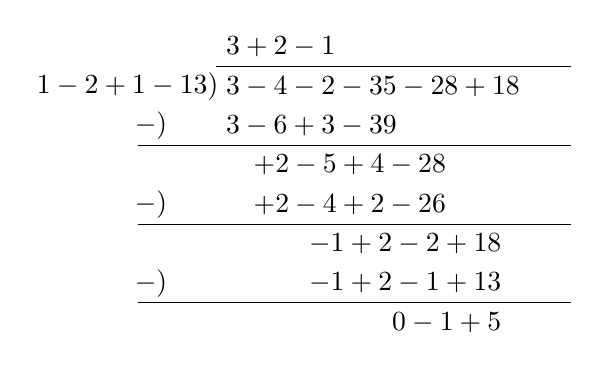
\begin{tikzpicture}
        \node at (0,0.5)[right]{$3+2-1$};
        \node at (0.15,0)[left]{$1-2+1-13)$};
        
        \node at (-.5,-0.5)[left]{$-)$};
        \node at (-.5,-1.5)[left]{$-)$};
        \node at (-.5,-2.5)[left]{$-)$};
        \draw (0,.25)--(4.5,.25);
    
        \node at (0,0)[right]{$3-4-2-35-28+18$};
    \node at (0,-.5)[right]{$3-6+3-39$};
    \draw (-1,-.75)--(4.5,-.75);
    \node at (0,-1)[right]{$\quad +2-5+4-28$};
    \node at (0,-1.5)[right]{$\quad +2-4+2-26$};
    \draw (-1,-1.75)--(4.5,-1.75);
    \node at (0,-2)[right]{$\qquad\quad -1+2-2+18$};
    \node at (0,-2.5)[right]{$\qquad\quad -1+2-1+13$};
    \draw (-1,-2.75)--(4.5,-2.75);
    \node at (0,-3)[right]{$\qquad\qquad\qquad 0-1+5$};
    \end{tikzpicture}  
\end{center}
    


所以,商式$Q(x)=3x^2+2x-1$,余式$R(x)=0x^2-x+5=-x+5$.这种简化形式的方法,叫做\textbf{分离系数法}.

\begin{example}
 试求$f(x)=5x^4-7x^3+10x^2-2x-3$除以$g(x)=x^2-1$的商式及余式.   
\end{example}

\begin{solution}
   长除法的书写格式,通常采用下列形式: 
\begin{center}
    \polylongdiv[style=D]{5x^4-7x^3+10x^2-2x-3}{x^2-1}
\end{center}
   

   因此,分离系数法就可以写成:
\begin{center}
    \begin{tikzpicture}
 \node at (0,.5) [right]{$5-7+10-2-3$};   
 \node at (0,0) [right]{$5+\;0\;-5$}; 
 \node at (0,-.5) [right]{\quad $-7+15-2$}; 
 \node at (0,-1) [right]{\quad $-7+\;0\;+7$}; 
 \node at (0,-1.5) [right]{\quad \qquad $15-9-3$}; 
 \node at (0,-2) [right]{\quad\qquad $15+\;0\;-15$}; 
\node at (0,-2.5)[right]{\quad\qquad\qquad $-9+12$};

\foreach \x in {-.25,-1.25,-2.25}
{
    \draw (-1, \x)--(4,\x);
    \node at (-.5, \x+.25){$-)$};
}
\node at (-1,.5){被除式:};
\node at (7,.5){除式};\node at (7,0){商式};
\node at (4.5,-2.5){余式};
\draw (4,.75)--(4,-.25);
\draw (4,.25)--(6,.25);
\node at (4,.5)[right]{$1+\;0\;-1$};
\node at (4,0) [right]{$5-7+15$};

\end{tikzpicture}
\end{center}

所以,商式$Q(x)=\polynomial[reciprocal]{5,-7,15}$,余式$R(x)=-9x+12$.
\end{solution}

应该注意:在长除法中,如果被除式的首项是$ax^n$,除式的首项是$bx^m$,那么,商式的首项就应该是$\frac{a}{b}x^{n-m},\; (n\ge m)$.

\begin{example}
已知被除式$f(x)$,除式$g(x)$,试用分离系数法求出商式$Q(x)$与余式$R(x)$:
\begin{enumerate}
    \item $f(x)=\polynomial[reciprocal]{2,-4,1,-3},\qquad g(x)=x-3$
    \item $f(x)=\polynomial[reciprocal]{2,-4,1,-3},\qquad g(x)=2(x-3)$
\end{enumerate}


\end{example}

\begin{solution}
     
  \begin{center}
         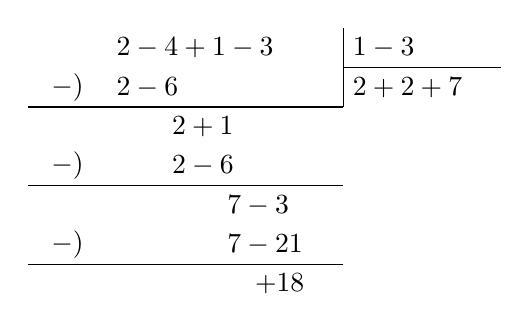
\begin{tikzpicture}
            \node at (0,.5) [right]{$2-4+1-3$};   
            \node at (0,0) [right]{$2-6$}; 
            \node at (0,-.5) [right]{\qquad $2+1$}; 
            \node at (0,-1) [right]{\qquad $2-6$}; 
            \node at (0,-1.5) [right]{\qquad \qquad $7-3$}; 
            \node at (0,-2) [right]{\qquad\qquad $7-21$}; 
           \node at (0,-2.5)[right]{\quad\qquad\qquad $+18$};
           
           \foreach \x in {-.25,-1.25,-2.25}
           {
               \draw (-1, \x)--(3,\x);
               \node at (-.5, \x+.25){$-)$};
           }
           
           \draw (3,.75)--(3,-.25);
           \draw (3,.25)--(5,.25);
           \node at (3,.5)[right]{$1-3$};
           \node at (3,0) [right]{$2+2+7$};
           
           \end{tikzpicture}
            \end{center}
  $\therefore\qquad Q(x)=\poly{2,2,7}$,$R(x)=18$.
  
  所以:$\poly{2,-4,1,-3}=(\poly{2,2,7})(x-3)+18$.


\begin{center}
    \begin{tikzpicture}
       \node at (0,.5) [right]{$2-4+1-3$};   
       \node at (0,0) [right]{$2-6$}; 
       \node at (0,-.5) [right]{\qquad $2+1$}; 
       \node at (0,-1) [right]{\qquad $2-6$}; 
       \node at (0,-1.5) [right]{\qquad \qquad $7-3$}; 
       \node at (0,-2) [right]{\qquad\qquad $7-21$}; 
      \node at (0,-2.5)[right]{\quad\qquad\qquad $+18$};
      
      \foreach \x in {-.25,-1.25,-2.25}
      {
          \draw (-1, \x)--(3,\x);
          \node at (-.5, \x+.25){$-)$};
      }
      
      \draw (3,.75)--(3,-.25);
      \draw (3,.25)--(5,.25);
      \node at (3,.5)[right]{$2-6$};
      \node at (3,0) [right]{$1+1+\tfrac{7}{2}$};
      
      \end{tikzpicture}
       \end{center}
$\therefore\qquad Q(x)=\poly{1,1,\frac{7}{2}}$,$R(x)=18$.

所以:$\poly{2,-4,1,-3}=\left(\poly{1,1,\frac{7}{2}}\right)\cdot 2(x-3)+18$.
\end{solution}

比较例4.37的两题,可以发现:两题的被除式相同,2题的除式是1题的除式的2倍,而相除的结果中得到:余式相同,2题的
商式却是1题商式的$\frac{1}{2}$.

这个规律,对多项式除法是正确的,这是因为:如果$f(x)=Q(x)\cdot g(x)+R(x)$成立,那么,$f(x)=\left[\frac{1}{a}Q(x)\right]\cdot [ag(x)]+R(x)$显然也成立.

因此,我们可以得出:

\begin{blk}{}
    两个多项式相除(除式不为0)时,如果被除式不变,而除式乘以一个非零常数$k$,那么,所得的余式不变,但商式却等于原
来商式的$\frac{1}{k}$.
\end{blk}

总结以上各例,可以归纳出一元多项式除法的原理和运算过程是:

把被除式、除式按降次排列成标准形式,逐步把除式乘以适当的单项式,使得每一次的积与被除式或“上一步所剩下来的式子”的首项相同,再相减就得到一个较低次数的多项式,这样逐步降次,直到
“所剩下来的式子”的次数低于除式的次数为止.
这时,“剩下来的式子”就是所求的余式,而每次所乘的单项式的代数和,就是所求的商式.

\begin{ex}
\begin{enumerate}
    \item 在下列各题中,$f(x)$是被除式,$g(x)$是除式,试用长除
    法、分离系数法求它们的商式与余式:
    \begin{enumerate}
        \item $f(x)=\poly{7,6,5,4,3,2,1,-7},\quad g(x)=\poly{1,1,-1}$
        \item $f(x)$同(a),$g(x)=x^2-1$
        \item $f(x)=\poly{1,0,3,0,1},\quad g(x)=\poly{2,0,3}$
        \item $f(x)=\poly{3,0,-5,0,-7,1,13},\quad g(x)=\poly{2,0,1,0,1}$
    \end{enumerate}

    \item 如果被除式$f(x)$是$n$次多项式,除式$g(x)$是$m$次多项
    式,你知道商式$Q(x)$, 余式$R(x)$是几次多项式吗?
    \item 先用分离系数法求$f(x)$除以$g(x)$的商式与余式,再不作
    除法,写出$f(x)$除以$\psi(x)$的商式与余式:
    \[f(x)=\poly{2,6,-4,0,-5},\qquad g(x)=x-2\]
\begin{enumerate}
    \item $\psi(x)=2(x-2)$
    \item $\psi(x)=\frac{1}{2}(x-2)$
\end{enumerate}

\end{enumerate}

\end{ex}



   \subsection{综合除法}
    以下介绍多项式$f(x)$除以$x-b$ ($b$为一个非零常数)的一种简便方法.
\begin{example}
    求$f(x)=2x^3+3x-1$ 除以$g(x)=x-4$的商式和余式.
\end{example}

\begin{solution}
用分离系数法,
\begin{center}
    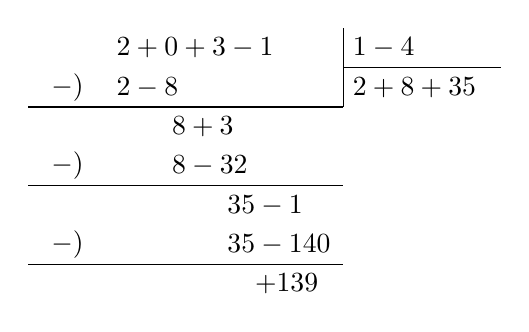
\begin{tikzpicture}
       \node at (0,.5) [right]{$2+0+3-1$};   
       \node at (0,0) [right]{$2-8$}; 
       \node at (0,-.5) [right]{\qquad $8+3$}; 
       \node at (0,-1) [right]{\qquad $8-32$}; 
       \node at (0,-1.5) [right]{\qquad \qquad $35-1$}; 
       \node at (0,-2) [right]{\qquad\qquad $35-140$}; 
      \node at (0,-2.5)[right]{\quad\qquad\qquad $+139$};
      
      \foreach \x in {-.25,-1.25,-2.25}
      {
          \draw (-1, \x)--(3,\x);
          \node at (-.5, \x+.25){$-)$};
      }
      
      \draw (3,.75)--(3,-.25);
      \draw (3,.25)--(5,.25);
      \node at (3,.5)[right]{$1-4$};
      \node at (3,0) [right]{$2+8+35$};
      
      \end{tikzpicture}
       \end{center}
$\therefore\quad $商式$Q(x)=\poly{2,8,35}$,余式$R(x)=+139$.

因为余式$R(x)$的次数要低于除式$g(x)$的次数,而这里的除式
$(x-4)$是一次式,所以,这里的余式就只能是零次多项式(非零数)或零多项式.在今后,对于除式是一次式的除法,所求得的余式,就直接说成是余数.
\end{solution}

把例4.38中的算式进一步分析一下,是可以发现其中的规律的:

\begin{center}
    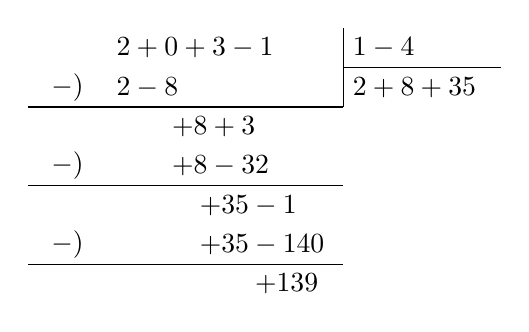
\begin{tikzpicture}
       \node at (0,.5) [right]{$2+0+3-1$};   
       \node at (0,0) [right]{$\boxed{2}-8$}; 
       \node at (0,-.5) [right]{\qquad $+8+3$}; 
       \node at (0,-1) [right]{\qquad $\boxed{+8}-32$}; 
       \node at (0,-1.5) [right]{\qquad \quad $+35-1$}; 
       \node at (0,-2) [right]{\qquad\quad $\boxed{+35}-140$}; 
      \node at (0,-2.5)[right]{\quad\qquad\qquad $+139$};
      
      \foreach \x in {-.25,-1.25,-2.25}
      {
          \draw (-1, \x)--(3,\x);
          \node at (-.5, \x+.25){$-)$};
      }
      
      \draw (3,.75)--(3,-.25);
      \draw (3,.25)--(5,.25);
      \node at (3,.5)[right]{$1-4$};
      \node at (3,0) [right]{$2+8+35$};
      
      \end{tikzpicture}
       \end{center}

\begin{enumerate}
    \item 除式$(x-4)$首项系数为1,因而商式的首项系数2,正好是被除式的首项系数.
    \item 在算式左半部分,凡被围的各数字,正好是商式的各项系数,它们除首项系数与被除式首项系数相同外,都和每一步“所剩下来的式子”的首项系数相同.
    \item 在算式左半部分,被围数字之后的一个数,分别是这样得到的:
    \[-8=\boxed{2}\x (-4),\quad -32=\boxed{8}\x(-4),\quad -140=\boxed{35}\x(-4) \]
它们有相类似的运算次序.
\item 如果将被围的数字,一律下移到最末一行,排列为:
\[\boxed{2}\quad \boxed{+8}\quad \boxed{+35}\; +139\]
那么,前三个数字就是商式的系数,末一个数就是余数.
\end{enumerate}
 

所以,上边的算式可以压缩化简为这样的形式:
\begin{center}
    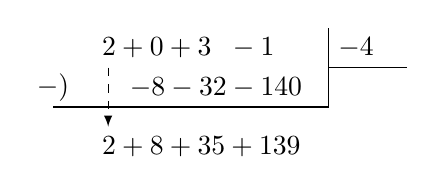
\begin{tikzpicture}[>=latex]
\node at  (0,0)[right]{\quad $-8-32-140$};
\node at  (0,.5)[right]{$2+0+3\;\;-1$};
\node at  (0, -.75)[right]{$2+8+35+139$};
\node at (-.5, 0){$-)$};
\draw [dashed,->](0.2,.25)--(0.2,-.5);
\draw (-.5, -.25)--(3,-.25);
\draw (3,-.25)--(3,.75);
\draw (3,.25)--(4,.25);
\node at (3,.5)[right]{$-4$};
    \end{tikzpicture}
\end{center}


为了计算方便,上式中的减法可以改为加法,这只要将减数$-8,-32,-140$改变符号就行,再由这些数的形成规律看,只要将$-4$改变符号,这些数的符号就相应地改变了.因而,上边的算式又可以进一步简化为:
\begin{center}
    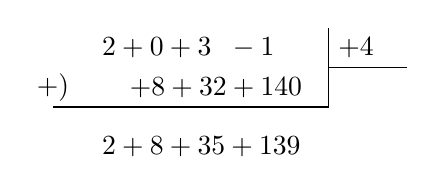
\begin{tikzpicture}
\node at  (0,0)[right]{\quad $+8+32+140$};
\node at  (0,.5)[right]{$2+0+3\;\;-1$};
\node at  (0, -.75)[right]{$2+8+35+139$};
\node at (-.5, 0){$+)$};
\draw (-.5, -.25)--(3,-.25);
\draw (3,-.25)--(3,.75);
\draw (3,.25)--(4,.25);
\node at (3,.5)[right]{$+4$};
    \end{tikzpicture}
\end{center}
这样就能得出:商式:$\poly{2,8,35}$,余数:$+139$.

\begin{example}
    求$f(x)=\poly{7,0,5,4,0,3,1}$除以$g(x)=x+3$的商式$Q(x)$及余数$R$
\end{example}

\begin{solution}
\[\because\qquad  g(x)=x+3=x-(-3)\]
\[f(x)=7x^6+0x^5+5x^4+0x^3+4x^2+3x+1\]
\begin{center}
  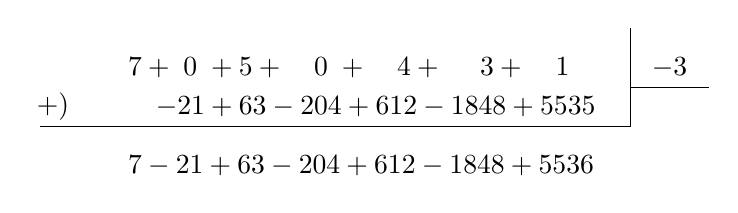
\begin{tikzpicture}
\node at (0,.5)[right]{$7+\;0\;+5+\quad 0\;+\quad 4+\quad\; 3+\quad 1$};
\node at (7,.5){$-3$};
\node at  (0,0) [right] {$\quad -21+63-204+612-1848+5535$};
\node at (-.5, 0)[left]{$+)$};
\draw (-1,-.25)--(6.5,-.25);
\node at (0,-.75) [right]{$7-21+63-204+612-1848+5536$};
\draw (6.5,-.25)--(6.5,1);
\draw (6.5,.25)--(7.5,.25);
\end{tikzpicture}  
\end{center}
$\therefore\quad $商式$Q(x)=\poly{7,-21,68,-204,616,-1845}$,余数$R=5536$.
\end{solution}

这种简化的带余除法,叫做\textbf{综合除法}.这种方法比长除法要简化得多.

\begin{example}
    用综合除法求$f(x)=a_2x^2+a_1x+a_0$ 除以$g(x)=x-b$的商式$Q(x)$,余数$R$.
\end{example}

\begin{solution}
    \begin{center}
        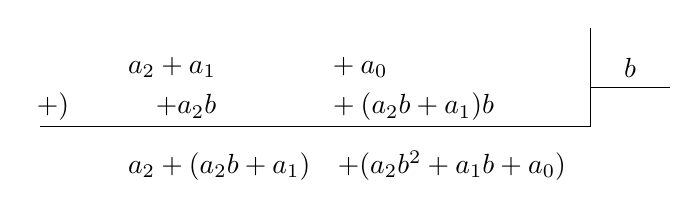
\begin{tikzpicture}
      \node at (0,.5)[right]{$a_2+a_1\qquad \qquad  +a_0$};
      \node at (6.5,.5){$b$};
      \node at  (0,0) [right] {$\quad +a_2b\qquad \qquad  +(a_2b+a_1)b$};
      \node at (-.5, 0)[left]{$+)$};
      \draw (-1,-.25)--(6,-.25);
      \node at (0,-.75) [right]{$a_2+(a_2b+a_1)\quad \uwave{+(a_2b^2+a_1b+a_0)} $};
      \draw (6,-.25)--(6,1);
      \draw (6,.25)--(7,.25);
      \end{tikzpicture}  
      \end{center}
$\therefore\qquad $ 商式$Q(x)=a_2x+(a_2b+a_1)$,余数$R=a_2b^2+a_1b+a_0$.
\end{solution}

如果除式$g(x)=px-q\quad (p\ne 0)$,可以先将除式变
形为:$px-q=p\left(x-\frac{q}{p}\right)$,用综合除法求出$f(x)$除以
$\left(x-\frac{q}{p}\right)$的商式$Q'(x)$及余数$R'$.它们满足关系式;
\[f(x)=Q'(x)\left(x-\frac{q}{p}\right)+R' \]
再根据前一节的结论可知:
\[\begin{split}
f(x)&=\frac{1}{p}Q'(x)\cdot p\left(x-\frac{q}{p}\right)+R'\\
&=\frac{1}{p}Q'(x)(px-q)+R'
\end{split}\]
因此,可以求得$f(x)$除以$(px-q)$的商式为:
$Q(x)=\frac{1}{p}Q'(x)$,余数为$R=R'$.

\begin{example}
    用综合除法求$f(x)$除以$g(x)$的商式及余数:
\begin{enumerate}
    \item $f(x)=\poly{6,13,27,15},\qquad g(x)=3x+2$
    \item $f(x)=\poly{8,7,-1},\qquad g(x)=4x-1$
\end{enumerate}    
\end{example}

\begin{solution}
\begin{enumerate}
    \item    $\because\quad g(x)=3x+2=3\left[x-\left(-\frac{2}{3}\right)\right]$

    $\therefore\quad $ 可先求$f(x)$除以$\left[x-\left(-\frac{2}{3}\right)\right]$的商式$Q'(x)$及余数$R'$.

    \begin{center}
        \begin{tikzpicture}
      \node at (0,.5)[right]{$6+13+27+15$};
      \node at (4.5,.5){$-\tfrac{2}{3}$};
      \node at  (0,0) [right] {\quad $-4\;\; -6\;\; -14$};
      \node at (-.5, 0)[left]{$+)$};
      \draw (-1,-.25)--(4,-.25);
      \node at (0,-.75) [right]{$6\; +9\;+21 \quad \uwave{+1}$};
      \draw (4,-.25)--(4,1);
      \draw (4,.25)--(5,.25);
      \end{tikzpicture}  
      \end{center}
这样得到:$Q'(x)=\poly{6,9,21}$,$R'=1$.

$\therefore\quad Q(x)=\frac{1}{3}Q'(x)=\poly{2,3,7}$,$R=R'=1$.

$\therefore\quad \poly{6,13,27,15}=(\poly{2,3,7})(3x+2)+1$.

\item $\because\quad g(x)=4x-1=4\left(x-\frac{1}{4}\right),\quad f(x)=8x^4+0+0+7x-1$
 
由综合除法
\begin{center}
    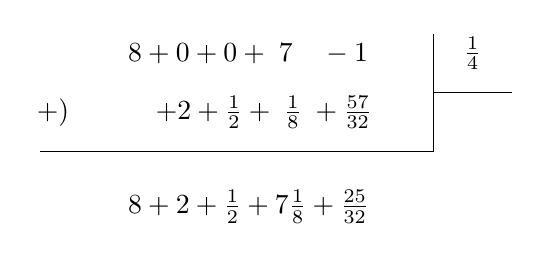
\begin{tikzpicture}
  \node at (0,.75)[right]{$8+0+0+\;7\quad -1$};
  \node at (4.5,.75){$\frac{1}{4}$};
  \node at  (0,0) [right] {\quad $+2+\frac{1}{2}+\;\frac{1}{8}\;+\frac{57}{32}$};
  \node at (-.5, 0)[left]{$+)$};
  \draw (-1,-.5)--(4,-.5);
  \node at (0,-1.2) [right]{$8+2+\frac{1}{2}+7\frac{1}{8}+\uwave{\frac{25}{32}}$};
  \draw (4,-.5)--(4,1);
  \draw (4,.25)--(5,.25);
  \end{tikzpicture}  
  \end{center}

  $\therefore\quad$ $f(x)$除以$g(x)$得商式
  \[\begin{split}
      Q(x)&=\frac{1}{4}\left(\poly{8,2,\frac{1}{2},7\frac{1}{8}}\right)\\
      &=\poly{2,\frac{1}{2},\frac{1}{8},\frac{57}{32}}
  \end{split}\]
  余数  $R=\frac{25}{32}$.
\end{enumerate}
\end{solution}

\begin{ex}
    用综合除法求商式及余数
\begin{enumerate}
    \item  $\poly{1,2,-14,54,-45,-378}$   除以   $x-3$  ;
    \item   $\poly{1,0,0,-3,2,-4}$  除以   $x+1$  ;
    \item   $\poly{9,0,-1,1,-3}$  除以   $5x-2$  ;
    \item   $\poly{8,2,0,4,-3,-1}$  除以   $2x+1$  ;
    \item  $\poly{6,-1,0,2,-1}$   除以   $\left(\frac{1}{3}x-1\right)$  ;
\end{enumerate}
\end{ex}


综合除法只是长除法过程的简化.对于除式是高于一次的多项式,仍可以类似进行.但书写较复杂,暂不研究.

一元多项式除法的基本原理在于进行逐步降次,
直到“所剩下来的式子”的次数低于除式的次数为止.对于多元多项式来说,一般地就不可能使各个未知数同时都降次,所以,多元多项式一般没有除法,从这个意义上来看,除法是一元多项式特有的一种运算.


\subsection{待定系数法求商式与余式}
待定系数法是根据多项式恒等的条件来解决问题的一种常用代数方法.以下就以求多项式的商式与余
式为例,说明这种方法.

\begin{example}
    试求
    $f(x)=\poly{3,1,-4,-17,5}$除以$g(x) =\poly{1,1,1}$的商式$Q(x)$与余式$R(x)$.
\end{example}

\begin{analyze}
    因为所求的商式$Q(x)$、余式$R(x)$一
定满足等式:$f(x)=Q(x)\cdot g(x)+R(x)$.

这里又已知$f(x)$是四次式,$g(x)$是二次式,不难判断,$Q(x)$一定是二次式,$R(x)$的次数低于二次,即$R(x)$的次数最高是一次.

因此,我们可以不作长除法,而设出:
$$Q(x)=ax^2+bx+c,\qquad R(x)=dx+e$$
其中$a,b,c,d,e$都是将要确定的系数,我们都叫做待定系数.

由除法的基本关系等式:
$$f(x)=Q(x)\cdot g(x)+R(x)$$
就可以利用多项式恒等条件,进而求出$a$、$b$、$c$、$d$、$e$的值,最后也就求出了商式及余式.
\end{analyze}

\begin{solution}
    由题意可设:
\[Q(x)=\poly{a,b,c},\qquad R(x)=dx+e\]

$\because\quad f(x)=Q(x)\cdot g(x)+R(x)$   

$\therefore\quad \poly{3,1,-4,-17,5}=(\poly{a,b,c})(\poly{1,1,1})+ax+e$

即:
\[\begin{split}
    &\quad \poly{3,1,-4,-17,5}\\
    &=\poly{a,(a+b),(a+b+c),(b+c+d),(c+e)};
\end{split}\] 
比较等式两边对应同类项的系数,得
\[\begin{cases}
    3=a\\
    1=a+b\\
    -4=a+b+c\\
    -17=b+c+d\\
    +5=c+e
\end{cases}\Rightarrow\quad  \begin{cases}
    a=3\\
    b=-2\\
    c=-5\\
    d=-10\\
    e=10
\end{cases}\]
所以,商式$Q(x)=\poly{3,-2,-5}$,余式$R(x)=-10x+10$.
\end{solution}

\begin{example}
    用待定系数法求$x^3+x^2+1$除以$2x^2+3x+1$所得的商式$Q(x)$及余式$R(x)$.
\end{example}

\begin{solution}
$\because\quad $ 被除式是3次式,除式是2次式,
$\therefore\quad $可设商式$Q(x)=ax+b$,
余式$R(x)=cx+d$.由于
\[x^3+x^2+1=(ax+b)(\poly{2,3,1})+(cx+d)\]
即:
\[x^3+x^2+1=\poly{2a, (3a+2b), (a+3b+c), (b+d)}\]
比较两边同类项系数可得:
\[\begin{cases}
  1=2a\\
  1=3a+2b\\
  0=a+3b+c\\
  1=b-d  
\end{cases}\Rightarrow\quad \begin{cases}
    a=\frac{1}{2}\\
    b=-\frac{1}{4}\\
    c=\frac{1}{4}\\
    d=\frac{5}{4}
\end{cases}\]
$\therefore\quad $商式$Q(x)=\frac{1}{2}x-\frac{1}{4}$,余式$R(x)=\frac{1}{4}x+\frac{5}{4}$.
\end{solution}

从以上两例可以看出,用待定系数法求多项式相除的商式及余式,其要点和原理是:
\begin{enumerate}
    \item 由被除式,除式的次数,设定商式与余式的
次数,并以待定系数形式设出它们的表达式.商式的次数为被除式与除式次数之差;余式次数可设为除式的次数减一.
\item 由于除法的基本等式
\[f (x) =Q (x) \cdot g (x) +R (x)\]
是恒等关系式,因此可以算出等式右边的结果.比较,两边同类项的系数,就得到以待定系数为未知数的方
程组.
\item 解方程组,就可以求得各待定系数,进而可
求得商式、余式.
\end{enumerate}

\begin{ex}
    用待定系数法求$f(x)$除以$g(x)$的商式及余式:
    \begin{enumerate}
        \item $f(x)=\poly{1,-3,1,3,-2},\qquad g(x)=\poly{1,-3,2}$
        \item $f(x)=\poly{3,0,-5,6, 1},\qquad g(x)=\poly{1,-3,4}$
    \end{enumerate}
\end{ex}

\section*{习题4.3}
\addcontentsline{toc}{subsection}{习题4.3}

\begin{enumerate}
    \item 计算:
\begin{enumerate}
    \item $(16m^2+24m^3)\div 8m^2$
    \item $(8a^3-12a^2+16a)\div (-4a)$
    \item $(ax^{n+4}-bx^{n+3}+cx^{n+2})\div x^2$
    \item $(3a^{n+2}+2a^{n+1}-4a^n)\div (-3a^{n-1})$
\item $(x-2)^2 \cdot (x+3)\div (x-2)$
\item $(3x-2)(5x+4)\div (2-3x)$
\end{enumerate}

\item 把$(x-2)$与$(x+b)$都看成一个整体,设为辅助未知数.试计算:
\begin{enumerate}
    \item $\left[4(x-2)^2+12(x+2)(x-2)-8(x-1)^2(x-2)\right]\div 4(x-2)$
    \item $\left[3(x+b)^3-6(x+b)^2+9(x+b)\right]\div 3(x+b)$
\end{enumerate}

\item 用分离变量法与待定系数法计算:

\begin{enumerate}
    \item $\poly{1,6,11,6,0}$ 除以 $x+3$;
    \item $\poly{1,6,11,6,0}$ 除以 $\poly{1,3,1}$;
    \item $\poly{1,2,-1,-2,1}$ 除以 $\poly{1,-1,1}$;
    \item $1-2x+8x^3-4x^2$ 除以 $4x^2-2$;
    \item $x+1+x^5+2x^3$ 除以 $2x+x^2+1$;
    \item $\poly{3,-5,-4,3,-2}$ 除以 $2x^2+x$.
\end{enumerate}

\item 用综合除法求$f(x)$除以$g(x)$的商式、余式.

\begin{enumerate}
    \item $f(x)=\poly{5,4,-12},\qquad g(x)=x+2$;
    \item $f(x)=\poly{3,-5,-4,3,-2},\qquad g(x)=x-2$;
    \item $f(x)=\poly{1,1,-3,4,-5,-6},\qquad g(x)=x-1$;
    \item $f(x)=\poly{2,1,-3,7,-5},\qquad g(x)=x-4$;
    \item $f(x)=x^8-1,\qquad g(x)=x+1$;
    \item $f(x)=x^2+6x^3-29x+21,\qquad g(x)=3x-2$;
    \item $f(x)=\poly{4,6,-8,-10},\qquad g(x)=2x-1$;
    \item $f(x)=\poly{3,-11,8,-3},\qquad g(x)=3x+2$;
    \item $f(x)=\poly{3,a,a^2,-2a^3},\qquad g(x)=3x-2a$;
    \item $f(x)=\poly{4,5b,9b^2,6b^3,4},\qquad g(x)=4x+b$.
\end{enumerate}

\item 已知$x^3+ax^2+bx+c=(x-1)(x-2)(x-3)+4$,试求:$a,b,c$的值.
\item 已知$f(x)=ax^4+bx^2+cx+d$的根是:$x_1=10$, $x_2=1$,
$x_3=12$, $x_4=4$.试求:$f(-1)$及$f\left(-\frac{1}{2}\right)$.
\item 如果已知$f(x)=8x^3-2x^2+ax+b$ 除以
$g(x)=4x^2-2$所得的余式为0,试求$a,b$的值.
\item 在第7题中,如果$f(x)$除以$g(x)$的余式是$5x-3$,
那么,$a$与$b$又是何值?
\item 试把多项式$3x^3-10x^2+13$表示成关于$(x-2)$的方
幂的形式.

\textbf{提示:} 先设$3x^3-10x^2+13=A(x-2)^3+B(x-2)^2
+C (x-2) +D$,即:
\[3x^3-10x^2+13=\{[A(x-2)+B](x-2)
+C\} (x-2)+D\]
再逐次用综合除法求出$D, C, B, A$.
\end{enumerate}



\section*{本章内容要点}

这一章的主要内容是多项式的有关概念及其四则运算.

一、由己知数与未知数符号的方幂相乘而得到的
式子叫单项式;若干个单项式的代数和,叫做多项式.多项式又叫做整式.

多项式的次数,就是指多项式中,次数最高的某一单项式的次数;而单项式的次数,就是所含各未知数的指数和.

任一非零常数,叫做零次多项式.

数零,叫做零多项式,它的次数不定.

\vskip 2ex 

二、一元$n$次多项式$f(x)$的标准形式是:
\[f (x) =a_n x^n +a_{n-1}x^{n-1}+\cdots+a_1x+a_0,\qquad (a_0\ne 0) \]
当$x=b$时,$f(x)$的值记作:
\[f (b) =a_n b^n +a_{n-1}b^{n-1}+\cdots +a_1b+a_0\]
\vskip 2ex 

三、两个多项式$f(x)$与$g(x)$,当$x$取任意值时,它们的值总相等,那么这两个多项式称为恒等,记作:
\[f (x) \equiv g (x) \]
如果$f(x)\equiv g(x)$,那么,这两个多项式相应的
同类项的系数都相等.这是待定系数法的依据.
\vskip 2ex 

四、能够使多项式$f(x)=0$的$x$的值,叫做多项式
$f(x)$的根.要求多项式$f(x)$的根,只要解方程$f(x)=0$就可以得到.
\vskip 2ex 

五、多项式的加、减,乘法运算的结果仍是多项
式(封闭的).而且具有数系运算的通性.
\vskip 2ex 

如果用$f,g$表示两个多项式(一元或多元),它
们分别为$m$次和$n$次($m>n$).那么,
\begin{itemize}
    \item $f+g$是一个$m$次多项式,$f-g$也是$m$次多项
    式;而$f\cdot g$是一个$(m+n)$次多项式.
\end{itemize}
\vskip 2ex 

六、常用乘法公式是运算的工具,必须掌握:
\[\begin{split}
    (a-b)(a+b)&= a^2-b^2\\
    (a\pm b)^2&=a^2\pm 2ab+b^2\\
    (a\pm b)^3&=a^3\pm 3a^2b+3ab^2\pm b^3\\
    (a\pm b)(a^2\mp ab+b^2)&=a^3\pm b^3
\end{split}\]

这些公式中的$a,b$,可以是数、或单项式、或多项式.因此,在应用中要具体分析,灵活掌握.
\vskip 2ex 

七、带余除法,是一元多项式的特有运算.

\begin{itemize}
    \item $f(x)$除以$g(x)$,就是要求出两个多项式$Q(x)$
    与$R(x)$,使它们满足关系式:
    \[f (x) =Q (x) \cdot g (x) +R (x)\]
    其中,$R(x)$的次数要低于$g(x)$的次数.
    \item 除法的原理是:逐步寻求单项式,进行降次
    工作.具体方法有:类似于整数除法的长除法、分离系数法、待定系数法以及除式为一次式的综合除法.
    \item 两个一元多项式相除,当除式乘以一个非零常数$k$时,所得商式就是原商式的$\frac{1}{k}$,所得余式不变,这是由于:
\[\begin{split}
    f(x)&=Q(x)\cdot g(x)+R(x)\\
    &=\frac{1}{k}Q'(x)\cdot [k\cdot g(x)]+R'(x)
\end{split}\]    

\end{itemize}


\section*{复习题四}
\addcontentsline{toc}{section}{复习题四}
\begin{enumerate}
    \item 计算:
    \begin{enumerate}
        \item $5x^2+(-4x)+1+(-3x)^2-(-5x)+(-3)^3+(-x^2)+6x-10$
        \item $4x^2y-(+5xy)+(-3x^2y)-(x^2y)^2-(-3x^3)-(-2xy)$
    \end{enumerate}
\item 有一串单项式:
\[-x,2x^2,-3x^3,4x^4,\ldots,-19x^{19},20x^{20},\ldots. \]
\begin{enumerate}
    \item 你能说出它们排列的规律吗?
    \item 根据你发现的规律,写出第100个、第101个、第
102个单项式来.
\item 你能写出第$n$个、第$n+1$个单项式来吗?
\end{enumerate}

\item 如果一个三元单项式的系数和次数都是4,试写出这
个单项式的表达式(要考虑所有符合条件的各种可能).
\item  有两个单项式,它们的和为$10x^2y$,它们的差为
$-6x^2y$.试求出这两个单项式.

\item 设$f(x)=\poly{3,-4,-5,1}$,$g(x)=\poly{2,1,4,-3}$,$h(x)=\poly{1,-1,-5,2}$
\begin{enumerate}
    \item 试计算:
    \[A=f(x)+g(x)+h(x),\qquad B=f(x)-g(x)+h(x)\]
    \[C=f(x)+g(x)-h(x),\qquad D=-f(x)+g(x)+h(x)\]
    \item 证明:$A=B+C+D$.
\end{enumerate}

\item 已知:$f(x)+2g(x)=\poly{-5,-3,2}$,且$2f(x)-g(x)=-x-1$.

试求出$f(x)$,$g(x)$的表达式.

\item 已知:$f(x)=ax^2+bx+c$的两个根为4,$-5$,且$f(1)=f(-1)+2$

试求:$f\left(\sqrt{2}\right)$,$f(10)$.

\item 试确定满足恒等式
$(\poly{a,b,c})(x^2+1)=\poly{2,6,-5,6,-7}$
的$a,b,c$的值.

\item 已知$f(x,y,z)=x^3+2(y^3+z^3)+6xyz$,求:$f(2,2,2)$.

\item 计算
\begin{enumerate}
    \item $\left(\frac{x}{\sqrt{2}}+1\right)\left(1-\frac{x}{\sqrt{2}}\right)$
    \item $\left(\sqrt{2}x+\sqrt{3}y\right)^2$
    \item $(x+2)^2+2(x-2)(x+2)+(x-2)^2$
    \item $(3x-2y+1)^2$
    \item $(5x^2-y^2)(-y^2-5x^2)$
    \item $(3x+y-2)(3x-y+2)-(3x-2)(3x+2)$
    \item $\left[(x^2-xy+y^2)(x^2+xy+y^2)\right]^2\cdot (x-y)^2\cdot (x+y)^2$
    \item $(a^8+b^8)\cdot (a+b)(a^4+b^4)(a-b)(a^2+b^2)$
\end{enumerate}

\item 利用乘法公式证明:
\[(x+y)^6=x^6+6x^5y+15x^4y^2+20x^3y^3+15x^2y^4+6xy^5+y^6\]
\item 如果$f(x)=\poly{1,2,a,b,1}$是一个二次多项式的完全平方式,试用待定系数法求$a,b$.
\item  试用综合除法求$f(x)$除以$(x-a)$的余数,并求出
$f (a)$:
\begin{enumerate}
    \item $f(x)=7x^5-3x^2+9$ 除以$x-2$ $(a=2)$;
    \item $f(x)=7x^5-3x^2+9$ 除以$x+1$ $(a=-1)$;
    \item $f(x)=4x^3-8x^2+3x-6$ 除以$x-\frac{1}{2}$ $(a=\frac{1}{2})$.
\end{enumerate}

\item 从上题的各小题中,你能发现各题的余数$R$与相应的$f(a)$有什么关系?再举一例,验证这一关系.
\item 试用综合除法求出下列各题中的$a$、$b$、$c$、$d$:
\begin{enumerate}
    \item $2x^2-x+1=a(x-1)^2+b(x-1)+c$;
    \item $x^3-6x^2+4x+8=a(x-1)^3+b(x-1)^2+c(x-1)+d$;
    \item $3x^3-8x^2+10=a(x-2)^3+b(x-2)^2+c(x-2)+d$.
\end{enumerate}
(参看习题4.3第9题提示).

\item 证明:
\begin{enumerate}
    \item 两个相邻奇数的平方差是8的倍数;
    \item 任意两个奇数的平方差除以8余0.
\end{enumerate}

\item 证明:
\begin{enumerate}
    \item $(x-y)(x^n+x^{n-1}y+\cdots +xy^{n-1}+y^n)=x^{n+1}-y^{n+1}$;
    \item $(x+y)(x^{2n}-x^{2n-1}y+\cdots -xy^{2n-1}+y^{2n})=x^{2n+1}+y^{2n+1}$
\end{enumerate}
\textbf{注:}第2题左边第二个括号内的符号是“$+$”、“$-$”相间.

\item  已知$ax^2+bx+c$是一个一次二项式的完全平方式.
试用待定系数法证明:$b^2-4ac=0$.
\item  如果$f(x)=6x^4-x^3-18x^2+x+12$,试证明$f(x)$
能写成下面的形式:
\[f(x)=(x-1)(x+1)(2x-3)(3x+4)\]
\item 已知$f(x+2)=\poly{3,20,45,50}$,试求:
    \begin{multicols}{2}
\begin{enumerate}
    \item $f(0)$;$f(-2)$
    \item $f(1)$;$f(-1)$
    \item $f(+10)$;$f(12)$
    \item $f(a)$;$f(-a)$
\end{enumerate}
\end{multicols}
\textbf{提示:}
\begin{enumerate}
    \item 可以将$\poly{3,20,45,50}$先写成以下形式:
    \[f(x+2)=A(x+2)^3+B(x+2)^2+C(x+2)+D\]
    再求值.
    \item 可以由$x+2=a$,求出$x=a-2$,直接代入原式求值.
\end{enumerate}

\end{enumerate}


